%%%%%%%%%%%%%%%%%%%%%%%%%%%%%%%%%%%%%%%%%%%%%%%%%%%%%%%%%%%%%%%%%%%%%%%%%
%
% File: operator_evolution.tex
%
% Author: A. J. Tropiano (tropiano.4@osu.edu)
% Date: August 23, 2019
%
% Draft of paper on SRG operator evolution and the Magnus expansion.
%
% Revision history:
%	08/28/19 --- Started outlining and added pieces from old notes.
%	09/27/19 --- Wrote the introduction.
%	11/15/19 --- Editing introduction, figures, and wrote the SRG potential evolution section.
%
%%%%%%%%%%%%%%%%%%%%%%%%%%%%%%%%%%%%%%%%%%%%%%%%%%%%%%%%%%%%%%%%%%%%%%%%%


\documentclass[preprintnumbers,floatfix,aps,prc,preprint,nofootinbib]{revtex4-1}

% Packages
\usepackage{amsmath}
\usepackage{amsfonts}
\usepackage{amssymb}
\usepackage{bm}
\usepackage[font=small,skip=0pt]{caption} % For captions on figures and tables
\usepackage{cellspace}
\usepackage{color}
\usepackage{enumerate}
\usepackage{epsfig}
\usepackage[figuresright]{rotating}
\usepackage{float}
\usepackage{hyperref} % For clickable links to sections within table of contents
\usepackage{graphicx}
\graphicspath{{../../Figures/}} % Setting the graphics path
\usepackage{physics} % For bra-ket notation
\usepackage{siunitx}
\usepackage[caption=false]{subfig} % For sub-figures

\newcommand{\eps}{\varepsilon}


\begin{document}


%%%%%%%%%%%%%%%%%%%%%%%%%%%%%%%%%%%%%%%%%%%%%%%%%%%%%%%%%%%%%%%%%%%%%%%%%
\title{Operator evolution from the similarity renormalization group and the Magnus expansion}


\author{A.~J.~Tropiano$^{1}$, S.~K.~Bogner$^{2}$, R.~J.~Furnstahl$^{1}$}

\affiliation{%
$^1$\mbox{Department of Physics, The Ohio State University, Columbus, OH 43210, USA}  \\
$^2$\mbox{Facility for Rare Isotope Beams and Department of Physics and Astronomy,}  \\
\mbox{Michigan State University, East Lansing, MI 48824, USA}
}

\date{\today}

\begin{abstract}

\noindent{Ideas for Magnus / SRG operator evolution paper}
\\
-- SRG/Magnus evolution in different potentials (non-local, local, semi-local). Universality. High cutoffs.
\\
-- Block-diagonal generator for high cutoff potentials and operator evolution. How the block-diagonal generator handles spurious bound states.
\\
-- Testing the Magnus expansion for high cutoff potentials using the potentials from Wendt 2011 for comparison. Spurious bound states and connection to intruder states in IMSRG calculations.
\\
-- Operator evolution for different potentials and generators.

\end{abstract}

\maketitle

\newpage


%%%%%%%%%%%%%%%%%%%%%%%%%%%%%%%%%%%%%%%%%%%%%%%%%%%%%%%%%%%%%%%%%%%%%%%%%
\section{Introduction}
\label{sec:intro}

% Unnecessary paragraph.
%\noindent{%
%\textbf{NN interaction and SRG decoupling.}
%}
%\\
%The nuclear many-body problem has long been hindered by the short-range repulsive core and strong tensor force in nucleon-nucleon (NN) interactions leading to non-perturbative few- and many-body systems and strongly correlated wave functions. The Fourier transform of NN interactions gives rise to the coupling of low- and high-momentum modes, which is manifested as non-zero off-diagonal potential matrix elements. It is very difficult to implement these interactions in many-body methods using basis expansions, because the matrix dimension becomes too large for accurate calculations. Renormalization group (RG) methods can be used to soften the interaction to make many-body methods feasible. One such method, the similarity renormalization group (SRG), allows for a continuous change in resolution of the potential without changing the observables. More generally, the SRG can evolve any operator and wave function for consistent calculation of observables.
%\\

Nuclear physics has seen a massive increase in the number of new NN interactions from chiral effective field theory ($\chi^{EFT}$) in the last decade. Previous SRG studies were limited to phenomenological interactions or the first non-local chiral interaction \cite{Entem:2003ft}, but with much more variety in modern chiral interactions, we would like to revisit the question of how different potentials and other operators change under SRG transformations. Since $\chi^{EFT}$ is an effective field theory, different potentials will still give the same $S$-matrix, that is, the potentials are phase equivalent up to some higher energy. However, the potentials themselves can differ in many ways such as the regulator functions, cutoff, order, and so forth, and thus, the potential matrix elements are not the same. Dainton \textit{et al.}~\cite{Dainton:2013axa} demonstrated SRG transformations drive different NN potentials to the same low-momentum matrix elements, that is, a flow to universality up to the momentum value of phase inequivalence. We address the question of universality for modern chiral potentials as well as how other operators change with respect to the corresponding SRG transformations.
\\

The SRG decouples low- and high-momentum scales in the Hamiltonian by applying a continuous unitary transformation $U(s)$ where $s=0 \rightarrow \infty$ is the flow parameter. An evolved operator is given by
%
\begin{eqnarray}
	\label{eq:srg_operator}
	O(s) = U(s) O(0) U^{\dagger}(s),
\end{eqnarray}
%
where $O(0)$ corresponds to the initial operator. Because $U(s)$ is unitary, the observables of the operator are preserved. In practice, the unitary transformation U(s) is not explicitly solved for; the evolved operator is given by solving a differential flow equation which is obtained by taking the derivative of Eqn. (\ref{eq:srg_operator}),
%
\begin{eqnarray}
	\label{eq:srg_flow}
	\frac{dO(s)}{ds} = [\eta(s), O(s)],
\end{eqnarray}
%
where $\eta(s)=\frac{dU(s)}{ds} U^{\dagger}(s) = -\eta^{\dagger}(s)$ is the anti-hermitian SRG generator. The generator is defined as a commutator, $\eta(s) = [G, H(s)]$, where $G$ specifies the type of flow and $H(s)$ is the evolved Hamiltonian. The choice in $G$ determines the pattern of decoupling in the Hamiltonian.
\\

By setting $G=H_D(s)$, the diagonal of the Hamiltonian, the Hamiltonian is driven to band-diagonal form. This choice was implemented by Wegner in condensed matter physics \cite{Wegner:1994ab}. In a similar option used in nuclear physics, $G$ is set to the relative kinetic energy, $T_{rel}$, which also drives to band-diagonal form. In most cases, these two choices give the same evolved operators. In exceptional cases, which will be discussed later in the paper, the two band-diagonal choices can have drastically different behavior. For band-diagonal decoupling, it is convenient to define $\lambda \equiv s^{-1/4}$ which roughly measures the width of the band-diagonal in the decoupled operator. For block-diagonal decoupling \cite{Anderson:2008mu}, 
%
\begin{eqnarray}
	\label{eq:block_diag_g}
	G =
	\begin{pmatrix}
		PH(s)P & 0 \\
		0 & QH(s)Q \\
	\end{pmatrix}
	\equiv H_{BD}(s),
\end{eqnarray}
%
where $P$ and $Q$ are low- and high-momentum projection operators, the Hamiltonian is split into low- and high-momentum sub-blocks by specifying a separation in momentum $\Lambda$ and taking $s \rightarrow \infty$. In momentum-space, the projection operators are step functions defined by the sharp cutoff in $\Lambda$. These transformations are similar to V\textsubscript{low $k$} transformations \cite{Bogner:2001gq, Bogner:2001jn, Bogner:2003wn} but keep the high-momentum matrix elements non-zero, although entirely decoupled from the low-momentum sub-block. Generally, the flow equation (\ref{eq:srg_flow}) is solved up to some finite value of $s$ with a high-order ODE solver. For notational convenience, we write the generators without the $s$ dependence in the rest of the paper.
\\

The decoupling of matrix elements does not necessarily hold in other operators as it does in the Hamiltonian. In a previous work \cite{Anderson:2010aq}, it was shown that SRG transformations induce low-momentum contributions in high-momentum operators and change very little in low-momentum operators. We investigate whether this is a general trend of the SRG for any potential and SRG generator. Instead of solving another set of flow equations, we apply SRG band- and block-diagonal transformations to other operators by building the unitary transformations explicitly using the eigenvectors of the initial and evolved Hamiltonians. SRG-evolved operators depend on the NN interaction despite having the same initial operator, since the flow equation (\ref{eq:srg_flow}) includes $H(s)$ from the definition of $\eta(s)$.
\\

There has also been renewed interest in studying chiral interactions at high cutoffs \cite{Tews:2018sbi}. In spin-triplet channels and at leading-order (LO), taking the cutoff to high values can result in spurious, deeply bound states from a highly singular short-ranged tensor force. In principle, these deep bound states are outside the range of the EFT and are absorbed by counterterms at higher order. In \cite{Wendt:2011qj}, it was shown that band-diagonal SRG decoupling of NN potentials in partial waves with spurious bound states differs significantly depending on the choice of SRG generator ($G=T_{rel}$ or $H_{D}$). These high cutoff potentials provide a test case to understand some of the previous points about universality, the choice of SRG generator and decoupling, as well as a good test problem for a variant of the SRG, which utilizes the Magnus expansion \cite{Morris:2015yna}.
\\

The Magnus expansion gives the SRG the capability to solve for the unitary transformation explicitly which can then be applied to any other operator of interest. This offers a huge numerical simplification in Fock-space where the matrix size of operators can become very large. The Magnus expansion is often used in in-medium SRG (IMSRG) calculations to solve the nuclear many-body problem directly. In some IMSRG calculations, intruder states can shift to the energy scale of the reference state in valence-space and severely distort low-energy properties. It is not understood how the IMSRG procedure evolves intruder state systems. Due to the prominence of the Magnus expansion in IMSRG, one must first understand if the Magnus approach matches the typical approach for difficult systems before investigating the intruder state problem. For this reason, NN potentials with spurious bound states offer a good test laboratory for the Magnus implementation to better understand if the Magnus is equivalent to the SRG approach.
\\

\noindent{%
\textcolor{red}{Overview of sections.}
}


%%%%%%%%%%%%%%%%%%%%%%%%%%%%%%%%%%%%%%%%%%%%%%%%%%%%%%%%%%%%%%%%%%%%%%%%%
\section{SRG evolution of NN potentials}
\label{sec:srg_evolution_nn_potentials}


%-- Fig.~\ref{fig:potential_contours_RKE_Wegner} illustrates the SRG in a nutshell. Here, we evolve three partial wave channels of RKE N$^4$LO \cite{Reinert:2017usi} where the cutoff $\Lambda=450$ MeV to $\lambda=1.5$ fm$^{-1}$. We see that the off-diagonal elements of the potential approach zero and the potential is driven to band-diagonal form.
%
% Unnecessary figure.
%\begin{figure}[H]
%	\centering
%	\subfloat[]{%
%	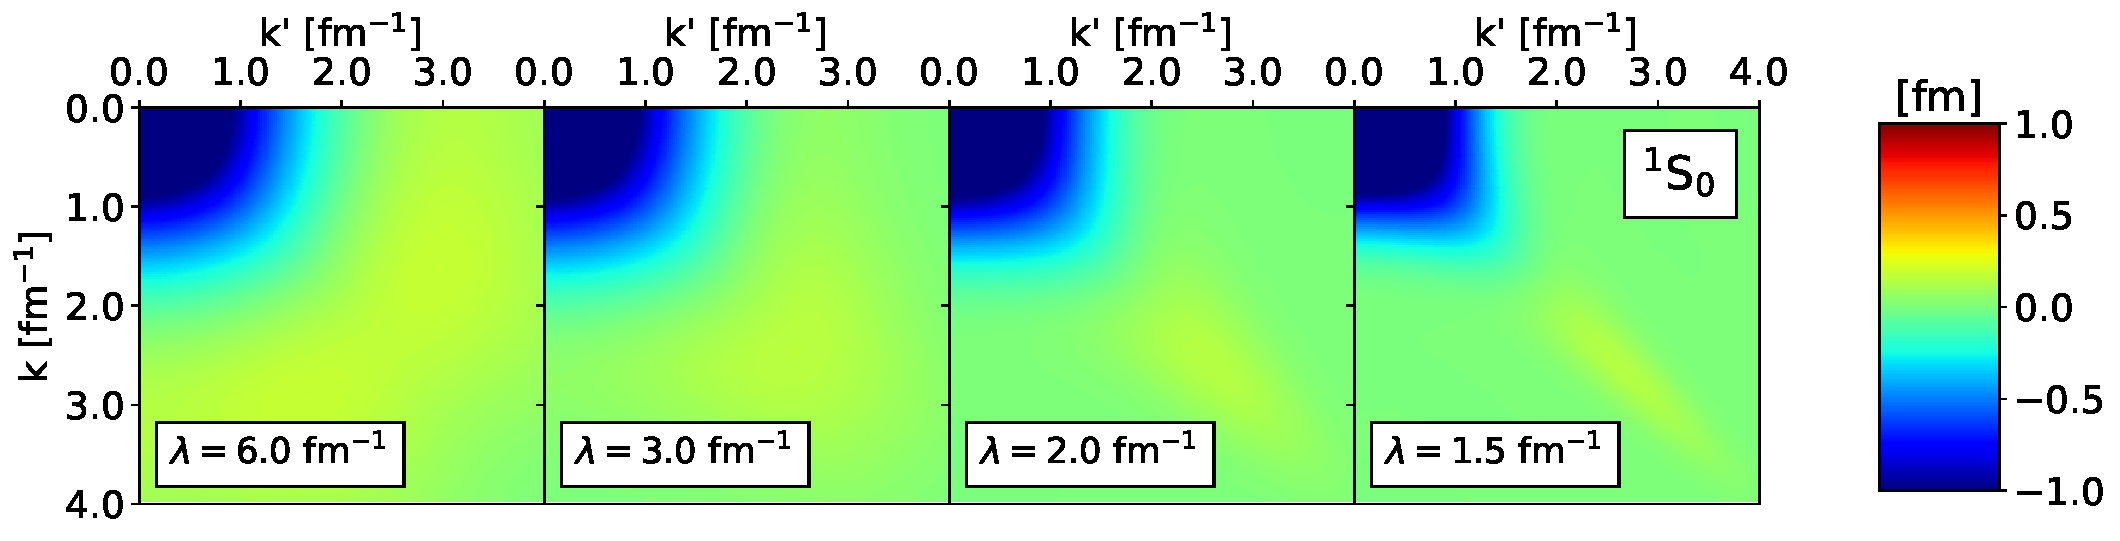
\includegraphics[clip,width=0.9\columnwidth]{SRG_potentials/potential_contours_kvnn111_1S0_Wegner_channel_label}%
%	}
	
%	\subfloat[]{%
%	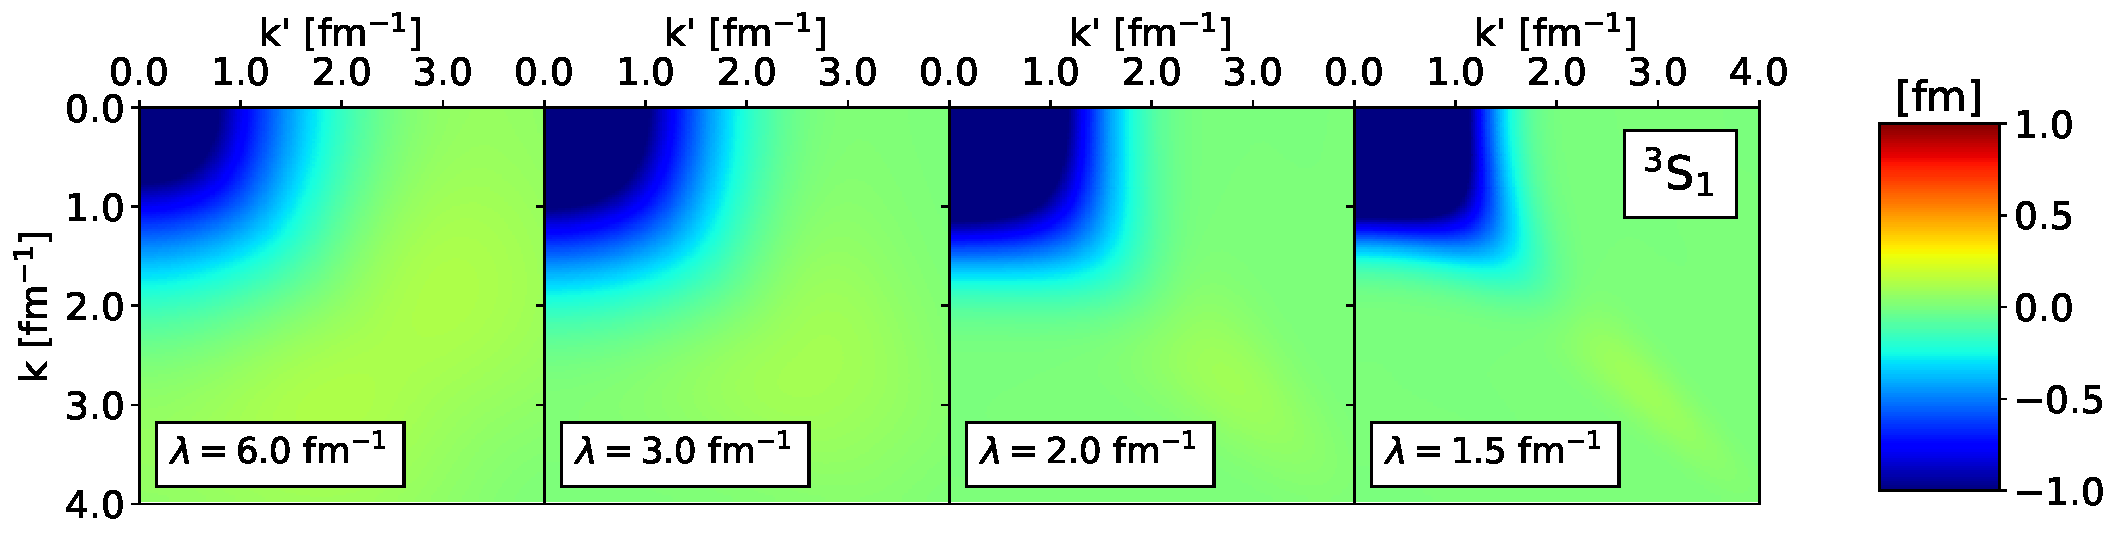
\includegraphics[clip,width=0.9\columnwidth]{SRG_potentials/potential_contours_kvnn111_3S1_Wegner_channel_label}%
%	}

%	\subfloat[]{%
%	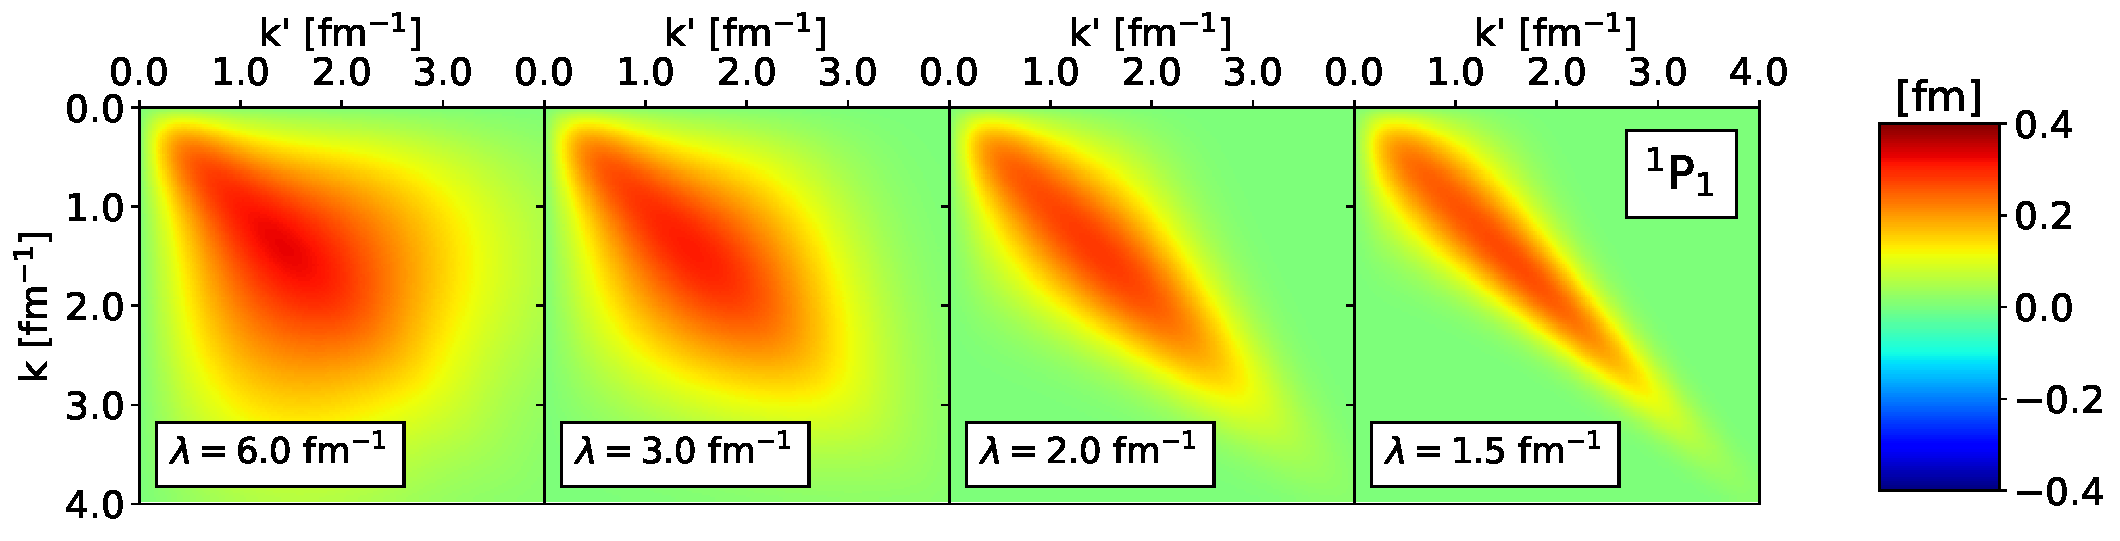
\includegraphics[clip,width=0.9\columnwidth]{SRG_potentials/potential_contours_kvnn111_1P1_Wegner_channel_label}%
%	}
%	\caption{Matrix elements of the RKE N$^4$LO potential SRG-evolving in $\lambda$ right to left under transformations with the Wegner generator in the $^1$S$_0$ (a), $^3$S$_1$ (b), and $^1$P$_1$ (c) channels.}
%	\label{fig:potential_contours_RKE_Wegner}
%\end{figure}
%
Here, we analyze SRG evolution of various chiral potentials with the Wegner band-diagonal generator and the block-diagonal generator. In Fig.~\ref{fig:potential_contours_3S1_Wegner} we show three different SRG-evolved potentials in the $^3$S$_1$ channel: EM N$^3$LO (500 MeV cutoff) \cite{Entem:2003ft}, RKE N$^4$LO (450 MeV cutoff) \cite{Reinert:2017usi}, and Gezerlis \textit{et al.}~N$^2$LO (1 fm cutoff) \cite{Gezerlis:2014zia}. A major difference in these three potentials are the regulator functions in the contact and pion-exchange terms. The EM N$^3$LO interaction is a non-local potential where both contact and pion-exchange interactions feature a non-local regulator function of the form exp$[-(k/\Lambda)^{2n}-(k'/\Lambda)^{2n}]$, where $\Lambda$ is the momentum-space cutoff and $n$ is an integer ($n=2$ in this case). However, a non-local regulator function for pion-exchange contributions can introduce regulator artifacts for cutoffs $\Lambda$ lower than the breakdown scale $\Lambda_b$. Several semi-local chiral potentials have been introduced to reduce regulator artifacts, such as the RKE potentials. Here, a local regulator function is applied for the long-range interactions in momentum-space, while a non-local regulator function is used for the short-range interactions. In some instances, non-local interactions are not suitable for $\textit{ab initio}$ approaches such as the quantum Monte Carlo (QMC) method motivating the need for fully local potentials. The Gezerlis \textit{et al.}~N$^2$LO potential is an example of a local interaction where the long-range terms have a local regulator function in coordinate-space and the short-range terms have a local regulator function in momentum-space.
%
\begin{figure}[H]
	\centering
	\subfloat[]{%
	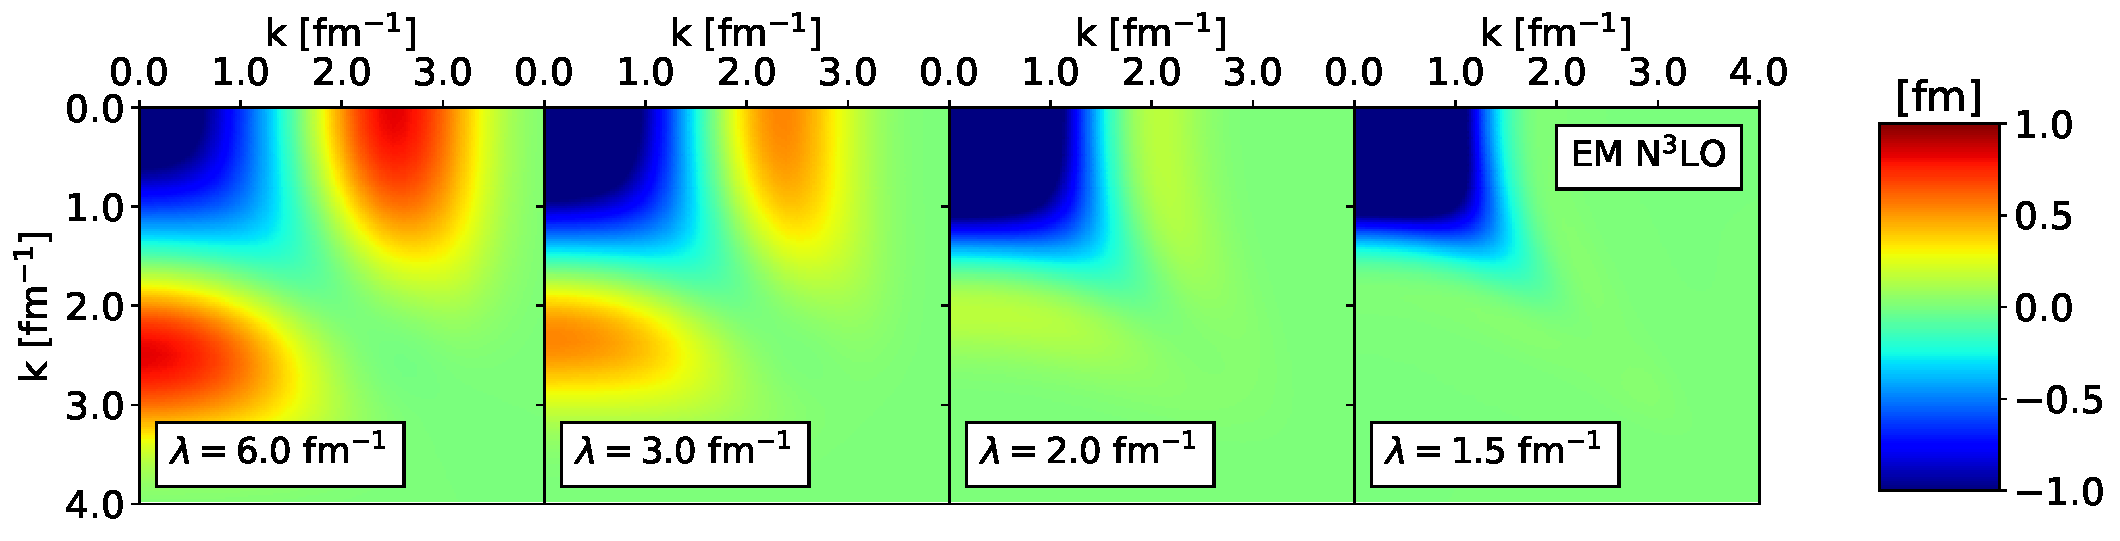
\includegraphics[clip,width=0.7\columnwidth]{SRG_potentials/potential_contours_kvnn10_3S1_Wegner_potential_label}%
	}
	
	\subfloat[]{%
	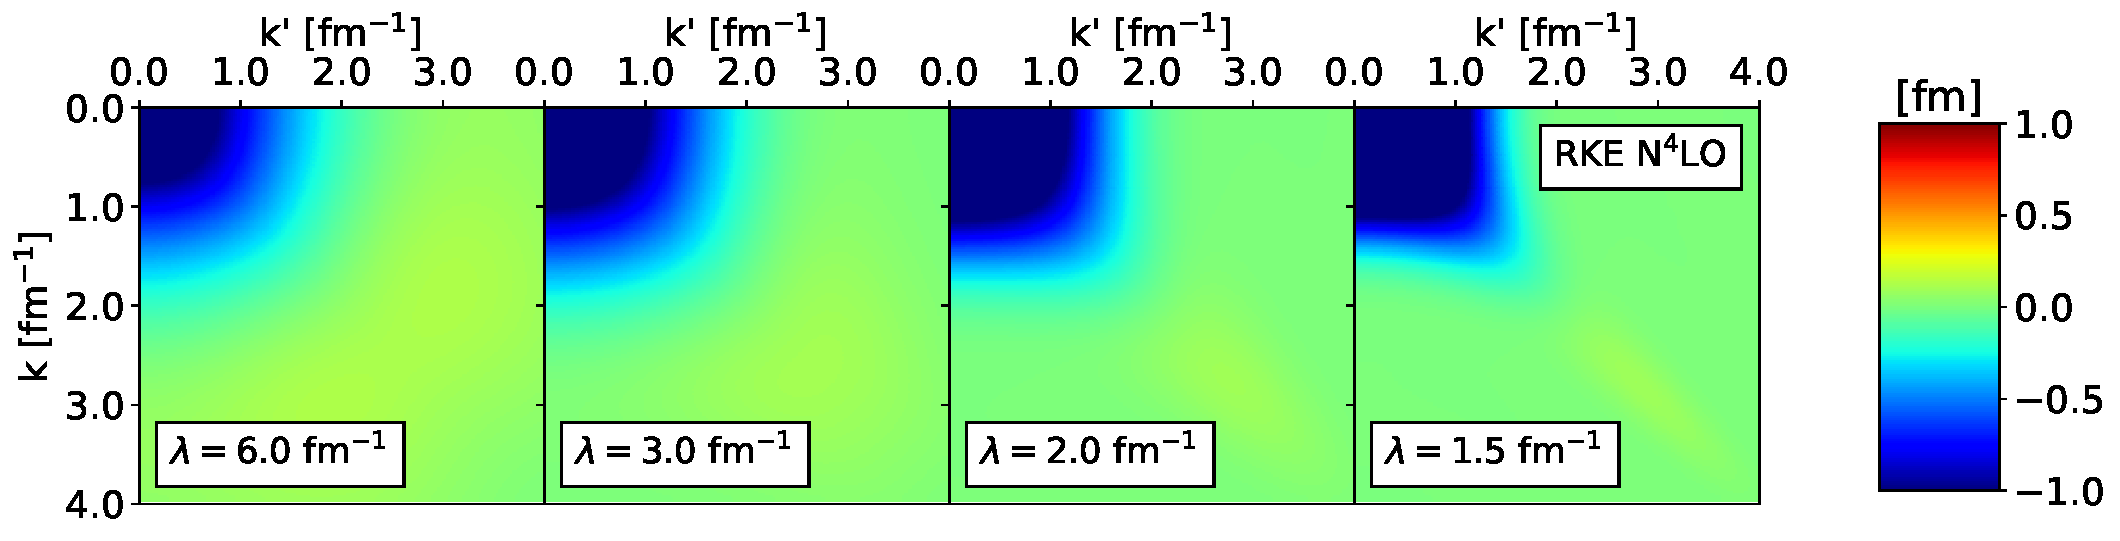
\includegraphics[clip,width=0.7\columnwidth]{SRG_potentials/potential_contours_kvnn111_3S1_Wegner_potential_label}%
	}

	\subfloat[]{%
	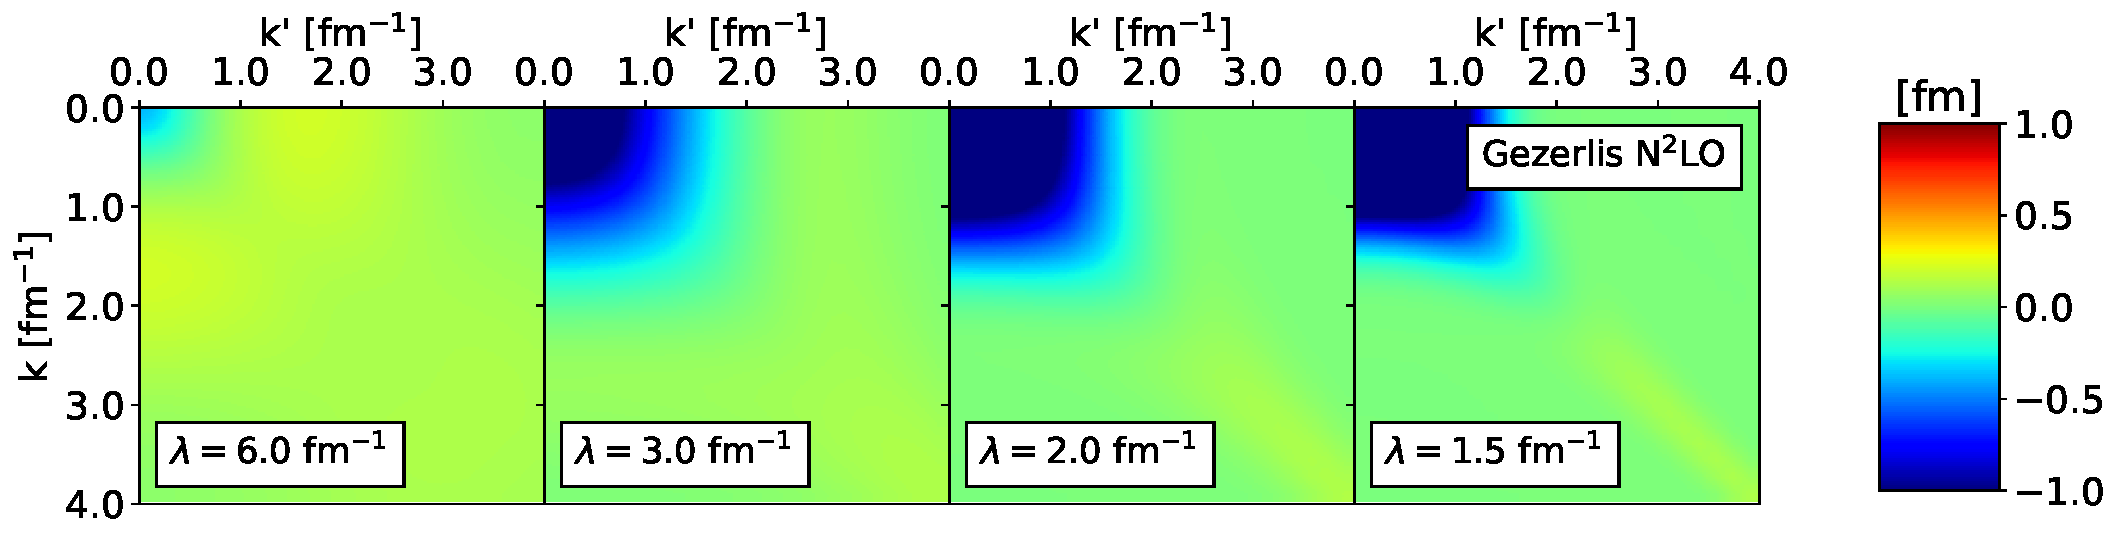
\includegraphics[clip,width=0.7\columnwidth]{SRG_potentials/potential_contours_kvnn222_3S1_Wegner_potential_label}%
	}
	\caption{Matrix elements of the EM N$^3$LO 500 MeV (a), RKE N$^4$LO 450 MeV (b), and Gezerlis \textit{et al.}~N$^2$LO 1 fm (c) potentials SRG-evolving in $\lambda$ right to left under transformations with the Wegner generator in the $^3$S$_1$ channel.}
	\label{fig:potential_contours_3S1_Wegner}
\end{figure}
%
These chiral interactions give the same low-energy phase shifts but the matrix elements of the potential are entirely different. In \cite{Dainton:2013axa}, with the SRG $T_{rel}$ generator, different phenomenological potentials were driven to universal low-momentum matrix elements. We see in Fig.~\ref{fig:potential_contours_3S1_Wegner} that the modern chiral potentials follow the same pattern. On the left-hand column where $\lambda=6$ fm$^{-1}$, the three potentials differ substantially. Further along the SRG evolution (right-hand side), the potentials are driven to band-diagonal form where the upper right corner of the contours, corresponding to low-momentum matrix elements, are the same. Note, we use the Wegner generator, $G=H_D$, in this SRG-evolution instead of $T_{rel}$ as in \cite{Dainton:2013axa}. For realistic nuclear interactions, these two band-diagonal choices are essentially the same. Only in extreme cases will there be a difference in the SRG-evolution.
%
\begin{figure}[H]
	\centering
	\subfloat[]{%
	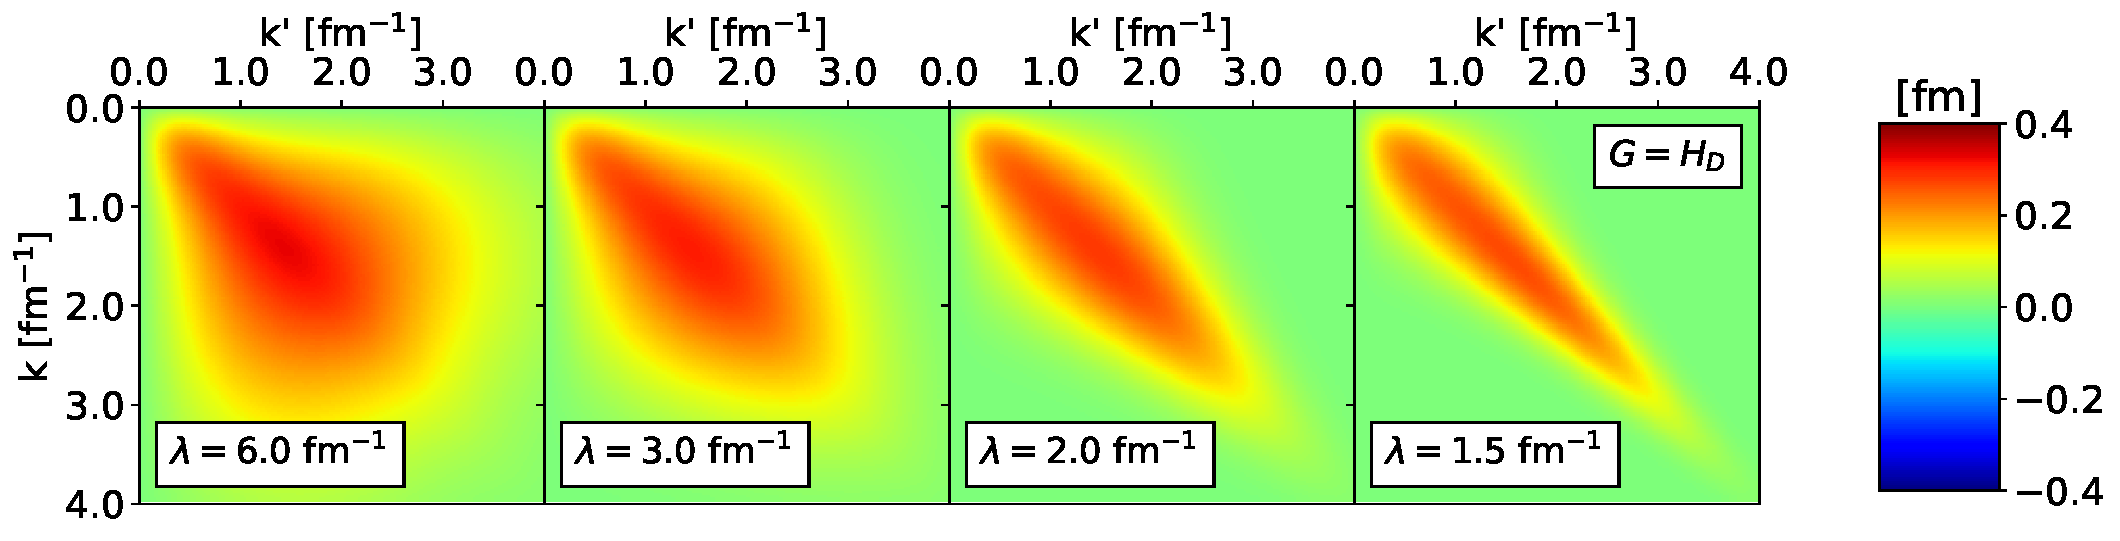
\includegraphics[clip,width=0.7\columnwidth]{SRG_potentials/potential_contours_kvnn111_1P1_Wegner_generator_label}%
	}
	
	\subfloat[]{%
	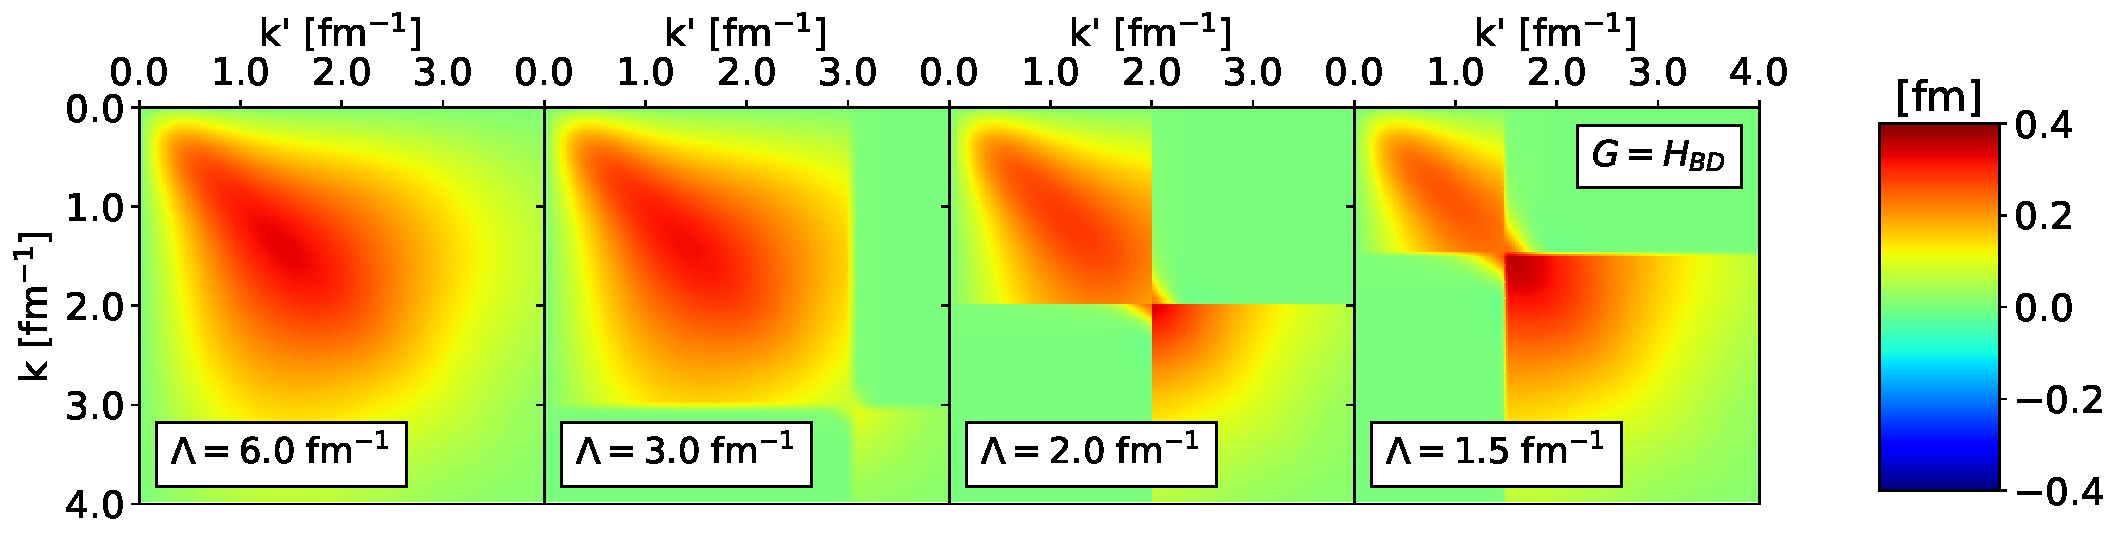
\includegraphics[clip,width=0.7\columnwidth]{SRG_potentials/potential_contours_kvnn111_1P1_Block-diag_generator_label}%
	}
	\caption{Matrix elements of the RKE N$^4$LO 450 MeV potential SRG-evolving right to left under transformations with Wegner (a) and block-diagonal (b) generators in the $^1$P$_1$ channel. Here, we use $\lambda$ for Wegner evolution in the top row and $\Lambda$ for block-diagonal evolution in the bottom row. For block-diagonal evolution, we fix $\lambda=1$ fm$^{-1}$.}
	\label{fig:potential_contours_1P1_RKE}
\end{figure}
%
Fig.~\ref{fig:potential_contours_1P1_RKE} shows the SRG-evolved RKE N$^4$LO (450 MeV cutoff) potential in the $^1$P$_1$ partial wave channel for band- and block-diagonal SRG generators on the top and bottom rows, respectively. We continue to evolve to band-diagonal form with respect to the parameter $\lambda$, but for the block-diagonal generator, we label sub-plots with the parameter $\Lambda$ which characterizes the sharp cutoff in decoupling the low- and high-momentum matrix elements. In the case of block-diagonal decoupling, one should take $s \rightarrow \infty$ which corresponds to $\lambda \rightarrow 0$. Of course, this is impossible numerically, so we take $\lambda=1$ fm$^{-1}$ for sufficiently decoupled sub-blocks. Thus, we see a small non-zero width in between the sub-blocks due to a non-zero value of $\lambda$. With block-diagonal decoupling, one can truncate the Hamiltonian at the value of $\Lambda$, separately diagonalize each sub-block, and retain all eigenvalues to high accuracy. We have tested several cases and acquired the same eigenvalues to less than roughly $.1$\% for both the low- and high-momentum sub-blocks.
%
\begin{figure}[H]
	\centering
	\subfloat[]{%
	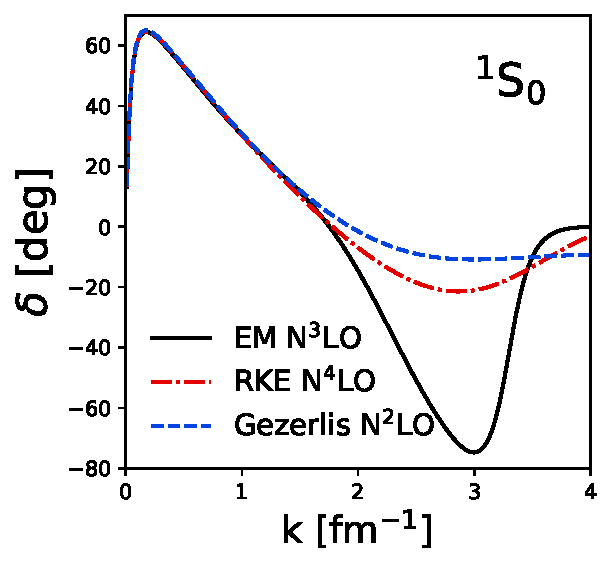
\includegraphics[clip,width=0.25\columnwidth]{SRG_observables/phase_shifts_1S0_kvnns_10_111_222}%
	}
	\quad
	\subfloat[]{%
	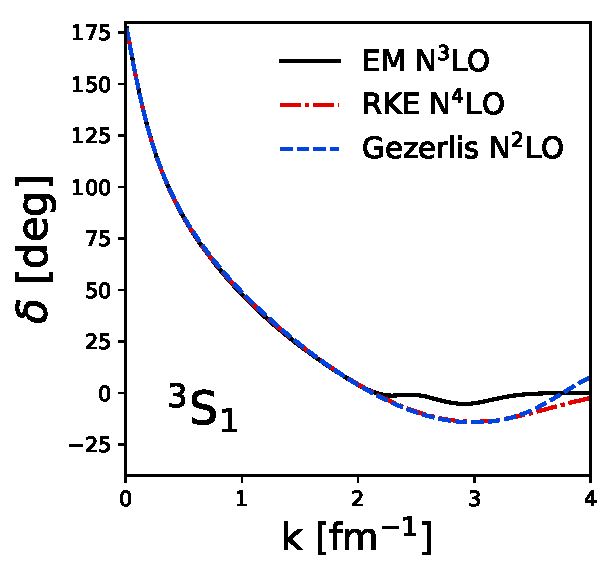
\includegraphics[clip,width=0.25\columnwidth]{SRG_observables/phase_shifts_3S1_kvnns_10_111_222}%
	}
	\quad
	\subfloat[]{%
	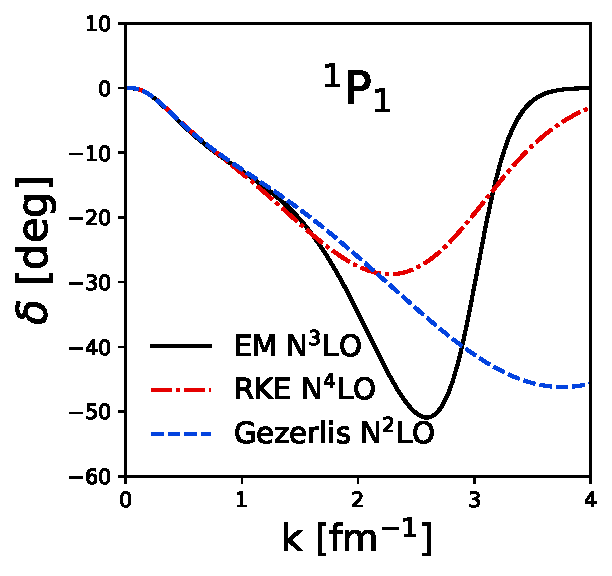
\includegraphics[clip,width=0.25\columnwidth]{SRG_observables/phase_shifts_1P1_kvnns_10_111_222}%
	}
	\caption{$^1$S$_0$ (a), $^3$S$_1$ (b), and $^1$P$_1$ (c) phase shifts for the EM N$^3$LO 500 MeV (solid black), RKE N$^4$LO 450 MeV (red dash-dotted), and Gezerlis \textit{et al.}~N$^2$LO 1 fm (blue dashed) potentials.}
	\label{fig:phase_shifts}
\end{figure}
%
In \cite{Dainton:2013axa}, it was found that phase equivalence up to some value of momentum $k$ implies potential matrix element equivalence up to the same value of $k$ in SRG-evolved potentials. We verify this conclusion for modern chiral potentials by checking the matrix elements in comparison to the phase shifts. Fig.~\ref{fig:phase_shifts} shows the NN phase shifts of EM N$^3$LO (500 MeV), RKE N$^4$LO (450 MeV), and Gezerlis \textit{et al.}~N$^2$LO (1 fm) potentials in the $^1$S$_0$, $^3$S$_1$, and $^1$P$_1$ partial wave channels. The phase shifts roughly agree up to some momentum value in the range $1-2$ fm$^{-1}$, and therefore, we expect the matrix elements of the SRG-evolved potentials to collapse up to these momentum values for each partial wave channel. To see this more quantitatively, we show the diagonal and far off-diagonal matrix elements of evolved potentials in Figs.~\ref{fig:potential_slices_1S0}, \ref{fig:potential_slices_3S1}, and \ref{fig:potential_slices_1P1}.
%
\begin{figure}[H]
	\centering
	\subfloat[]{%
	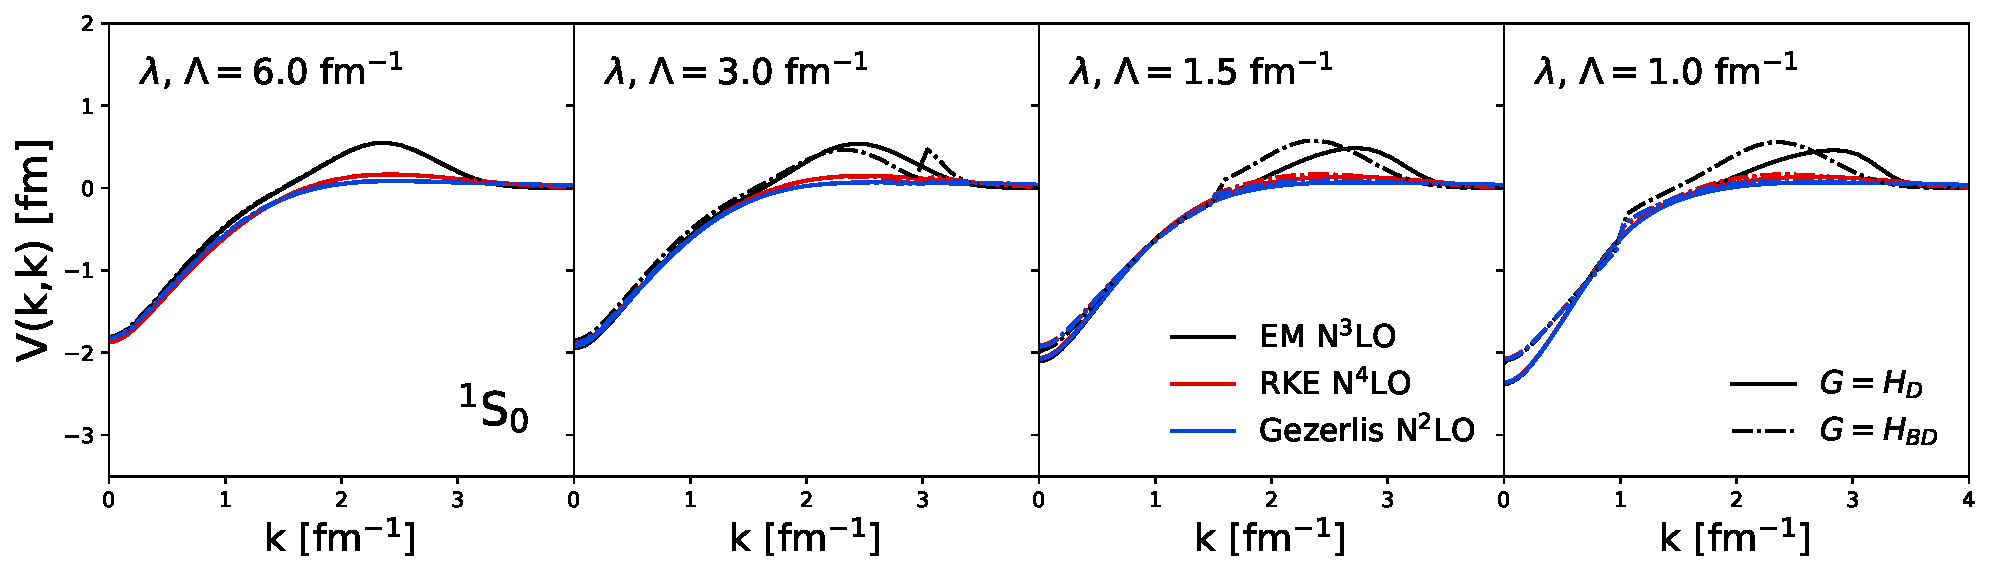
\includegraphics[clip,width=0.7\columnwidth]{SRG_potentials/potential_diag_1S0_kvnns_10_111_222_lamb1,0}%
	}
	
	\subfloat[]{%
	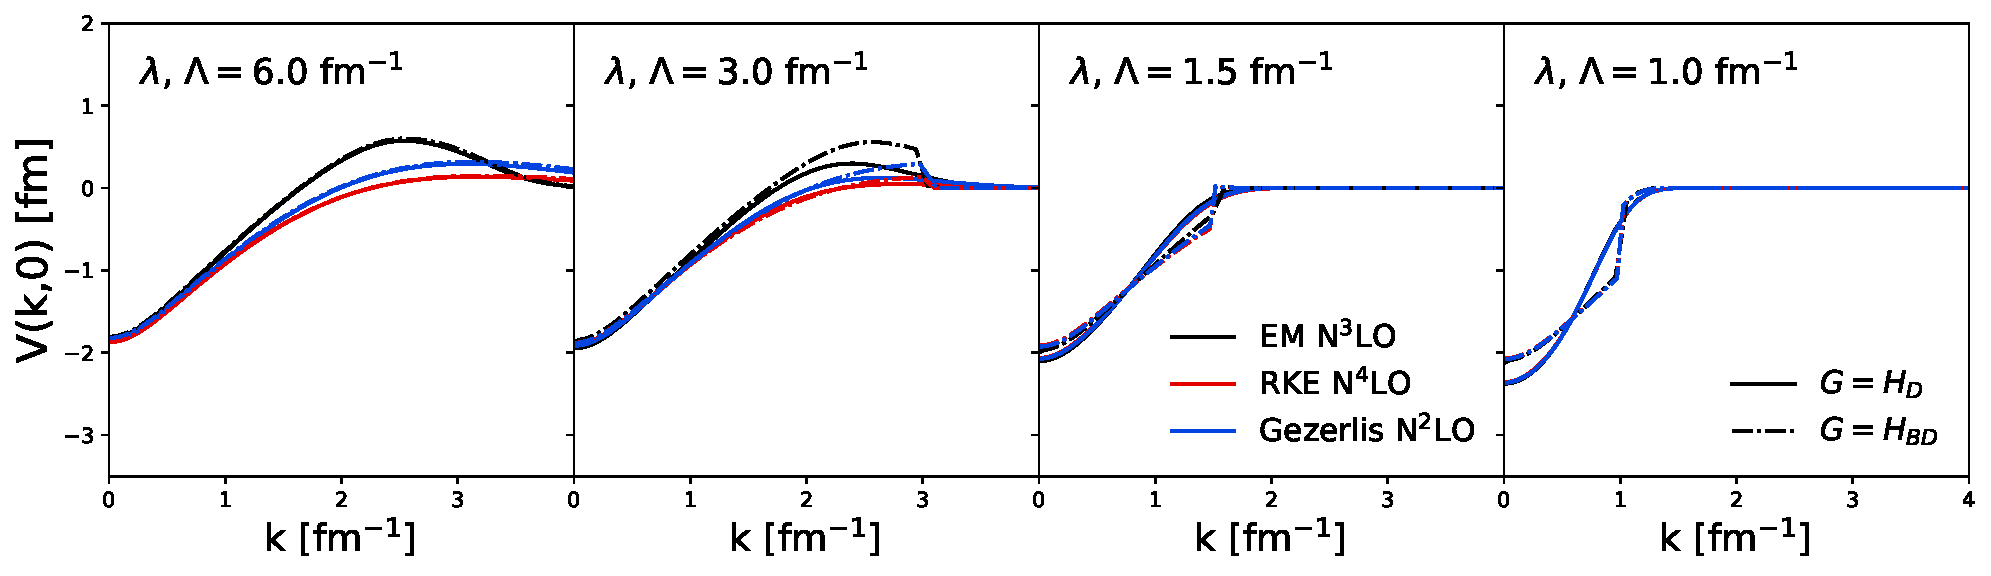
\includegraphics[clip,width=0.7\columnwidth]{SRG_potentials/potential_off-diag_1S0_kvnns_10_111_222_lamb1,0}%
	}
	\caption{Diagonal (a) and far off-diagonal (b) matrix elements of the EM N$^3$LO 500 MeV (black), RKE N$^4$LO 450 MeV (red) and Gezerlis \textit{et al.}~N$^2$LO 1 fm (blue) potentials SRG-evolving right to left under transformations with Wegner (solid) and block-diagonal (dashed) generators in the $^1$S$_0$ channel. Here, we use $\lambda$ for Wegner evolution and $\Lambda$ for block-diagonal evolution. For block-diagonal evolution, we fix $\lambda=1$ fm$^{-1}$.}
	\label{fig:potential_slices_1S0}
\end{figure}
%
In each of these figures, we show the diagonal matrix elements on the top row and the far off-diagonal matrix elements on the bottom row. (Note, in Fig.~\ref{fig:potential_slices_1P1}, the bottom row shows $V(k,0.5)$ instead of $V(k,0)$ because the far off-diagonal matrix elements in the $^1$P$_1$ channel are all zero.) Band- and block-diagonal evolved potentials are shown on the same plots indicated by solid and dashed lines, respectively, where the color indicates the potential. In the case of band-diagonal decoupling, as $\lambda$ is driven to a lower value than the $k$ value of phase shift equivalence, the low-momentum potential matrix elements collapse to the same line. For block-diagonal decoupling, the agreement only occurs for momentum-values less than the sharp cutoff $\Lambda$ where $\lambda$ is fixed to 1 fm$^{-1}$. The two generators collapse the potential to a different form, because the induced contributions from SRG flow depend on how the potential is decoupled, that is, the choice in $G$. In the $^3$S$_1$ channel (Fig.~\ref{fig:potential_slices_3S1}), we see a slight deviation in the lowest momentum potential matrix element from EM N$^3$LO and the other two potentials. This is due to a minor difference in the deuteron binding energy ($\approx 1\%$ difference). We will see in the next section that bound states significantly impact universality in SRG decoupling.
%
\begin{figure}[H]
	\centering
	\subfloat[]{%
	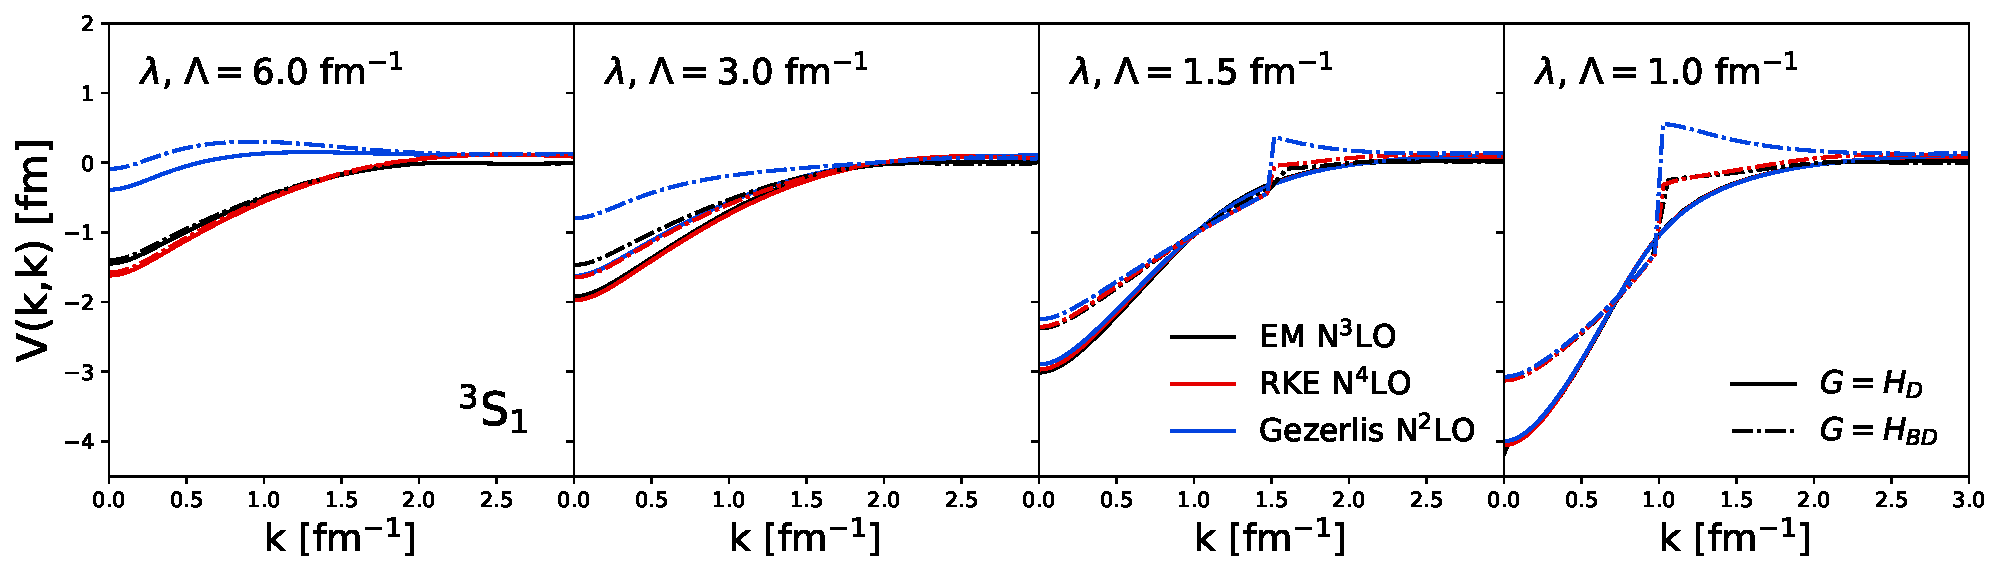
\includegraphics[clip,width=0.7\columnwidth]{SRG_potentials/potential_diag_3S1_kvnns_10_111_222_lamb1,0}%
	}
	
	\subfloat[]{%
	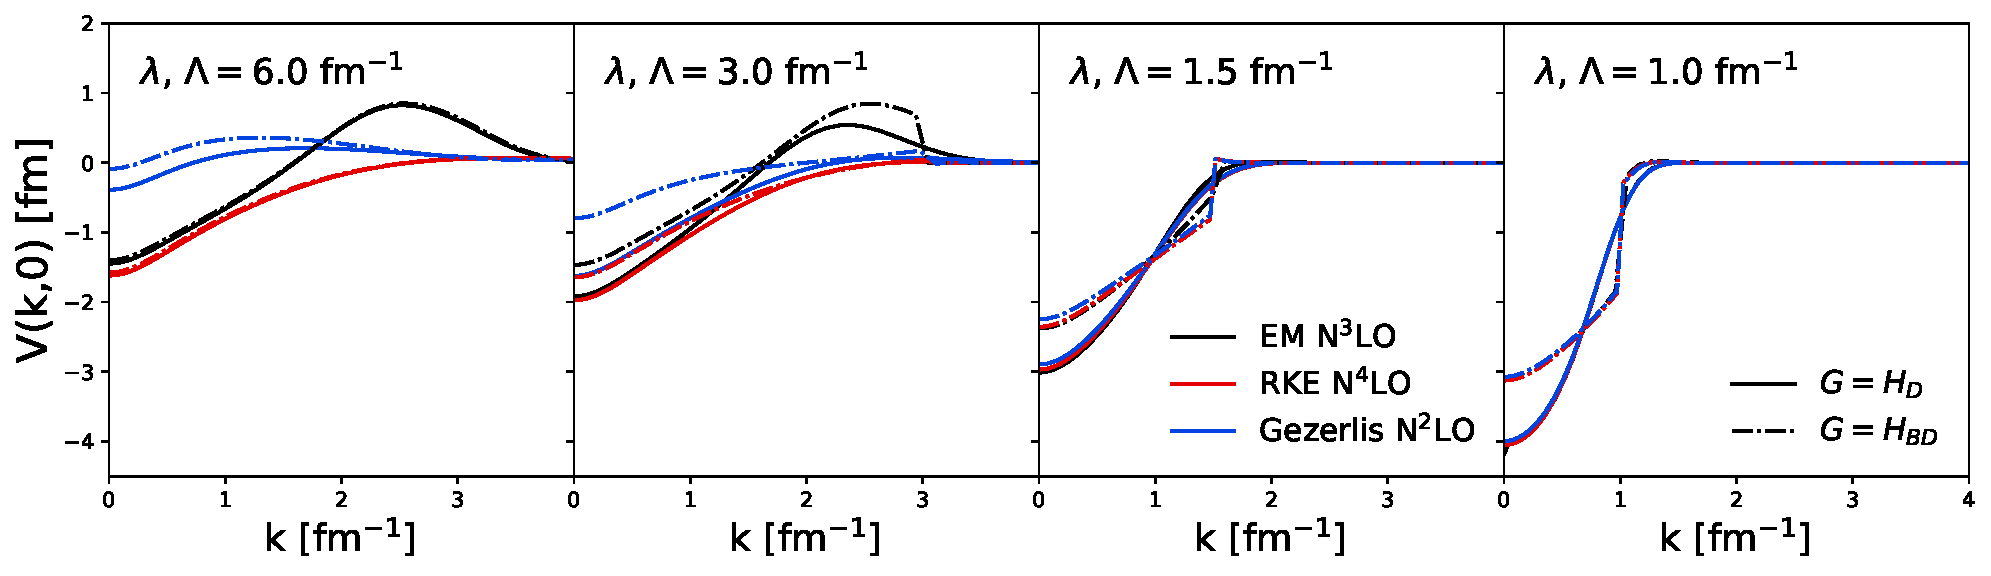
\includegraphics[clip,width=0.7\columnwidth]{SRG_potentials/potential_off-diag_3S1_kvnns_10_111_222_lamb1,0}%
	}
	\caption{Same as Fig.~\ref{fig:potential_slices_1S0} but in the $^3$S$_1$ channel.}
	\label{fig:potential_slices_3S1}
\end{figure}
%
\begin{figure}[H]
	\centering
	\subfloat[]{%
	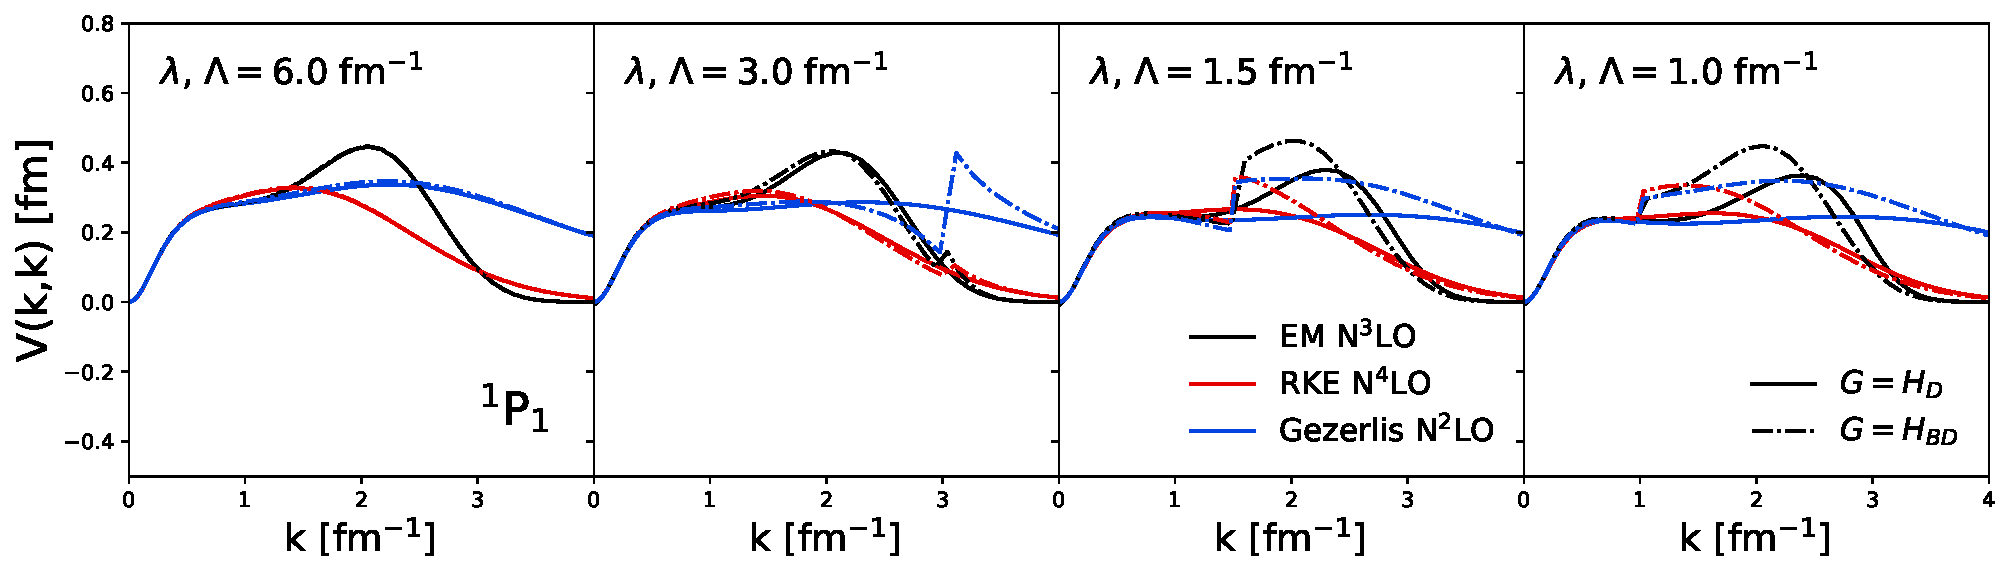
\includegraphics[clip,width=0.7\columnwidth]{SRG_potentials/potential_diag_1P1_kvnns_10_111_222_lamb1,0}%
	}
	
	\subfloat[]{%
	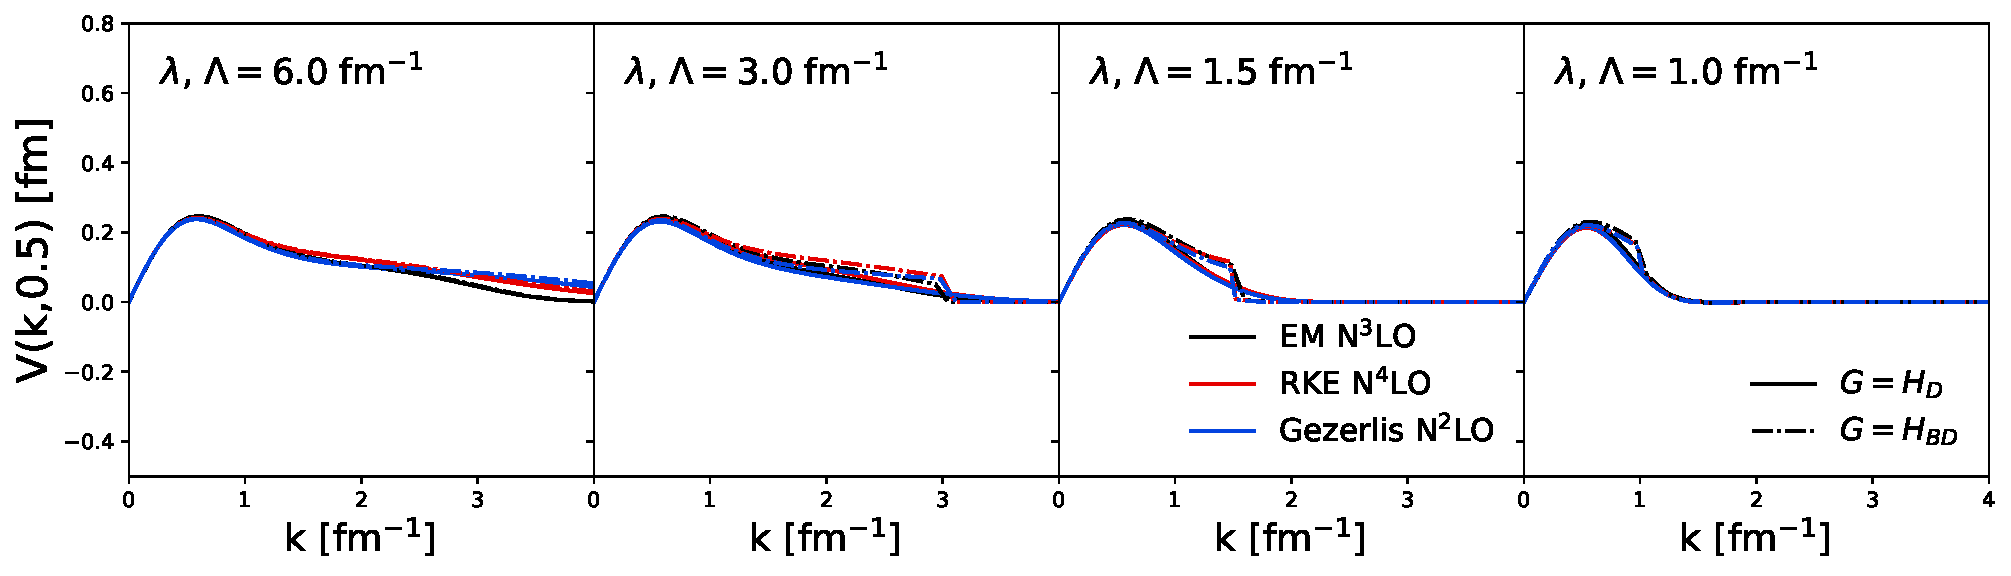
\includegraphics[clip,width=0.7\columnwidth]{SRG_potentials/potential_off-diag_1P1_kvnns_10_111_222_lamb1,0}%
	}
	\caption{Same as Figs.~\ref{fig:potential_slices_1S0} and \ref{fig:potential_slices_3S1} but in the $^1$P$_1$ channel.}
	\label{fig:potential_slices_1P1}
\end{figure}
%
\textcolor{red}{Updated up to here.}


%%%%%%%%%%%%%%%%%%%%%%%%%%%%%%%%%%%%%%%%%%%%%%%%%%%%%%%%%%%%%%%%%%%%%%%%%
\section{High cutoffs and the Magnus expansion}
\label{sec:high_cutoffs_magnus_exp}


% - - - - - - - - - - - - - - - - - - - - - - - - - - - - - - - - - - - - - - - - - - - - - - - - - - - - - - - - - - - - - - - - - - - - - - - - - - - - - - - - - - - - - - - - - - - - - - - - - - - - - - - - 
\subsection{High cutoffs and spurious bound states}
\label{sec:high_cutoffs}


\begin{itemize}
	\item Cutoff dependence in non-local LO (Wendt) potential. Recap of Wendt.
	\item Band- and block-diagonal evolution and universality. Add figure analogous to Fig.~\ref{fig:potential_slices_3S1} but for $\Lambda=4$, $9$, and $20$ fm$^{-1}$.
	\item Spurious bound state(s). Discussion on how the block-diagonal generator handles spurious bound states. Where they are ``decoupled'' in the matrix compared to Wegner. One figure to show this?
	\item Transition to Magnus expansion.
\end{itemize}
%
\begin{figure}[H]
	\centering
	\subfloat[]{%
	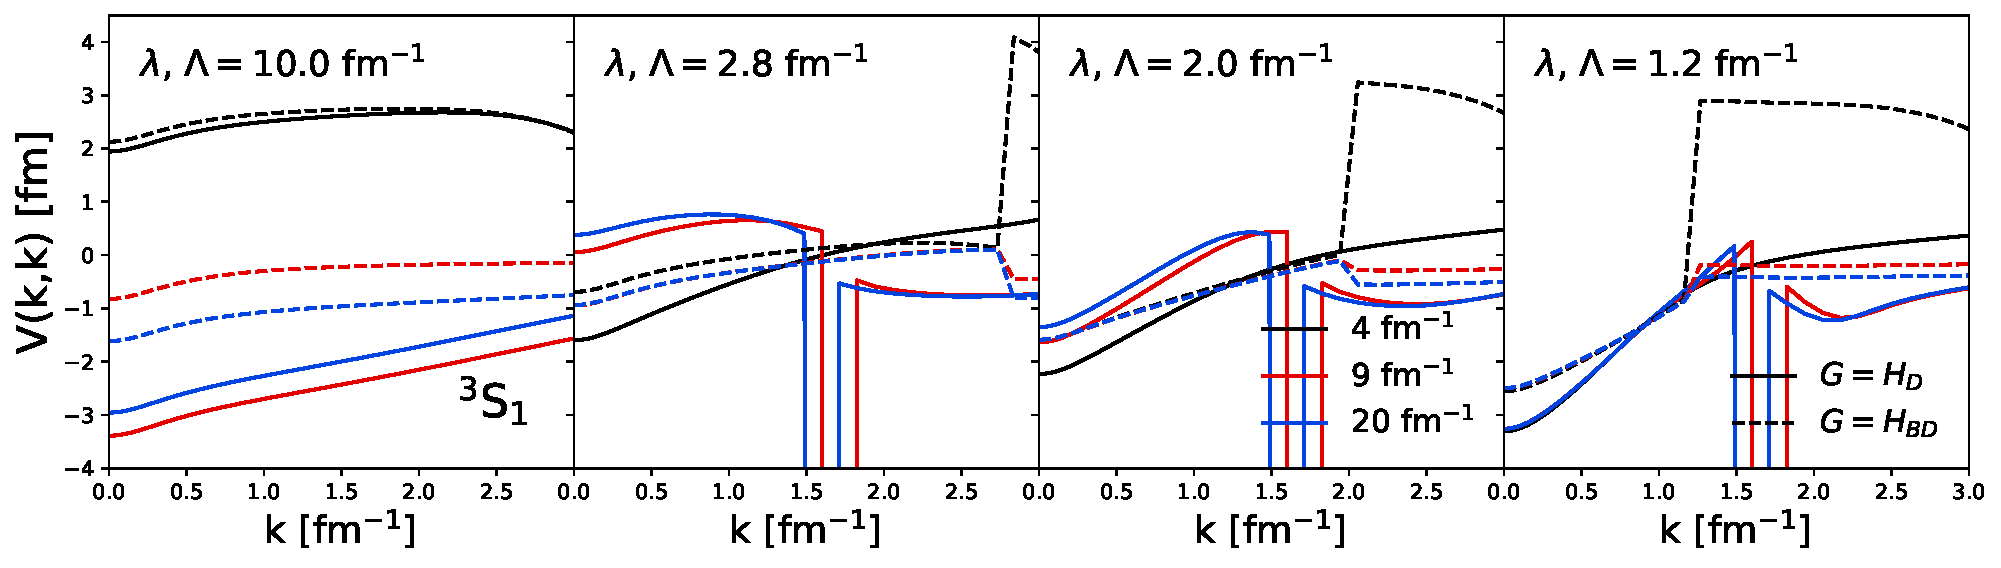
\includegraphics[clip,width=0.7\columnwidth]{SRG_potentials/potential_diag_3S1_kvnns_900_901_902_lamb1,2}%
	}
	
	\subfloat[]{%
	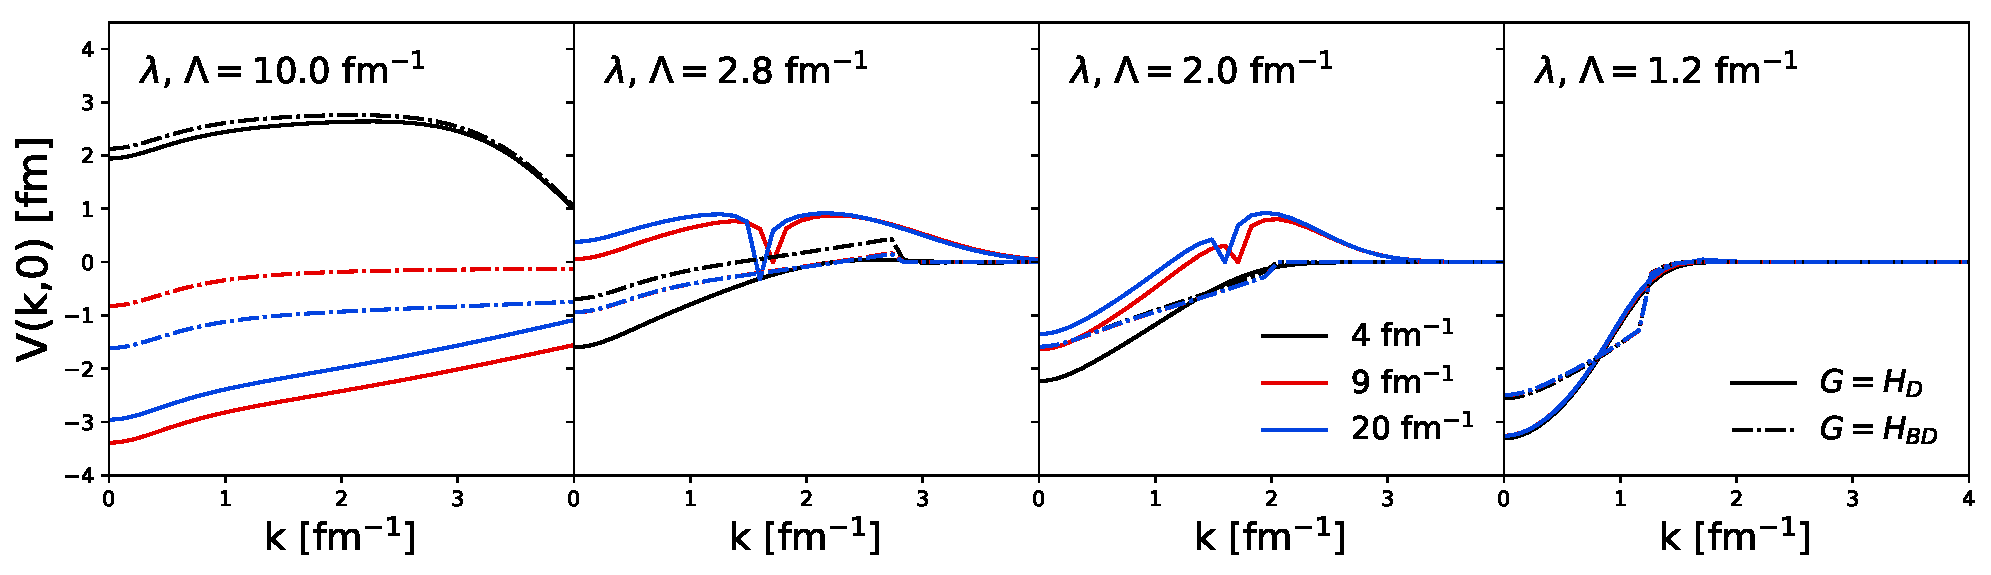
\includegraphics[clip,width=0.7\columnwidth]{SRG_potentials/potential_off-diag_3S1_kvnns_900_901_902_lamb1,2}%
	}
	\caption{Diagonal (a) and far off-diagonal (b) matrix elements of the non-local LO potentials at cutoffs $\Lambda=4$ (black), $9$ (red) and $20$ (blue) fm$^{-1}$ SRG-evolving right to left under transformations with Wegner (solid) and block-diagonal (dashed) generators in the $^3$S$_1$ channel. Here, we use $\lambda$ for Wegner evolution and $\Lambda$ for block-diagonal evolution. For block-diagonal evolution, we fix $\lambda=1.2$ fm$^{-1}$.}
	\label{fig:potential_slices_high_cutoffs}
\end{figure}
%


% - - - - - - - - - - - - - - - - - - - - - - - - - - - - - - - - - - - - - - - - - - - - - - - - - - - - - - - - - - - - - - - - - - - - - - - - - - - - - - - - - - - - - - - - - - - - - - - - - - - - - - - - 
\subsection{The Magnus expansion: Formalism}
\label{sec:magnus_expansion_formalism}

% What was said in the introduction: The Magnus expansion gives the SRG the capability to solve for the unitary transformation explicitly which can then be applied to any other operator of interest. This offers a huge numerical simplification in Fock-space where the matrix size of operators can become very large. The Magnus expansion is often used in in-medium SRG (IMSRG) calculations to solve the nuclear many-body problem directly.
\noindent{%
-- Motivation: simplifies computational problem for evolving multiple operators, exact unitarity.
}
\\
-- We now consider the Magnus implementation.
\\
-- Mathematically speaking, the Magnus expansion is a method for solving an initial value problem associated with a linear ordinary differential equation (ODE).
\\
-- Formal details of the Magnus expansion are discussed in \cite{Blanes:2009ab}.
\\
-- We will introduce the Magnus expansion in the context of SRG evolving any operator.
\\
-- In an intermediate step in deriving Eqn. (\ref{eq:srg_flow}), we have a linear ODE for $U(s)$,
%
\begin{eqnarray}
	\label{eq:unitary_trans}
	\frac{dU(s)}{ds} = \eta(s) U(s).
\end{eqnarray}
%
-- Magnus showed that one can solve the following equation with a solution $U(s)=e^{\Omega(s)}$ where $\Omega(s)$ is expanded as a power series, $\sum_{n}^{\infty} \Omega_n$ (referred to as the Magnus expansion or Magnus series).
\\
-- The terms of the series are given by integral expressions involving $\eta(s)$ (again, see \cite{Blanes:2009ab, Magnus:1954zz} for details).
\\
-- For our case, we focus on the formally exact derivative of $\Omega(s)$,
%
\begin{eqnarray}
	\label{eq:magnus_omega}
	\frac{d\Omega(s)}{ds} = \sum_{k=0}^{\infty} \frac{B_k}{k!} ad_{\Omega}^{k}(\eta),
\end{eqnarray}
%
where $B_k$ are the Bernoulli numbers, $ad_{\Omega}^{0}(\eta)=\eta(s)$, and $ad_{\Omega}^{k}(\eta)=[\Omega(s),ad_{\Omega}^{k-1}(\eta)]$.
\\
-- We integrate this differential equation to find $\Omega(s)$ and evaluate the unitary transformation directly.
\\
-- Then the evolved operator can be evaluated with the BCH formula:
%
\begin{eqnarray}
	\label{eq:bch}
	O(s) = e^{\Omega(s)} O e^{-\Omega(s)} = \sum_{k=0}^{\infty} \frac{1}{k!} ad_{\Omega}^{k}(O).
\end{eqnarray}
%
-- As $k \rightarrow \infty$ in both sums in Eqns. (\ref{eq:magnus_omega}) and (\ref{eq:bch}) the Magnus transformation matches the SRG transformation exactly.
\\
-- We investigate several truncations $k_{max}$ in Eqn. (\ref{eq:magnus_omega}) and take many terms, $k_{max} \sim 25$, in Eqn. (\ref{eq:bch}).
\\
-- There are significant advantages in the Magnus implementation.
\\
-- In the typical approach, the numerical error associated with solving the flow equation affects the accuracy of the observables for the evolved operator.
\\
-- Therefore, one must use a high-order ODE solver in integrating the flow equation (\ref{eq:srg_flow}).
\\
-- In the Magnus implementation, unitarity is guaranteed by the form of $U(s)$; in fact, one could solve Eqn. (\ref{eq:magnus_omega}) with a simple first-order Euler step-method keeping the same observables while decoupling the operator as desired.
\\
-- This offers a decent computational speed-up by avoiding a high-order solver.
\\
-- In this paper, we demonstrate this advantage by applying the Magnus implementation using the first-order Euler step-method.
\\
-- The second major advantage involves the evolution of multiple operators.
\\
-- In many other situations, one may be interested in evolving several operators at a time.
\\
-- In the SRG procedure, we would have another set of coupled equations in Eqn. (\ref{eq:srg_flow}), drastically increasing memory usage.
\\
-- Each additional operator increases the set of equations - say $N$ equations - by another factor of $N$.
\\
-- In the Magnus, one only needs $\Omega(s)$ to consistently evolve several operators.
\\
-- We avoid the cost in memory by directly constructing $U(s)=e^{\Omega(s)}$.
\\
-- This is especially useful in IMSRG calculations where the model space can be very large.
\\
-- We discuss results from Magnus-evolved large-cutoff potentials focusing on the flow of the potential, observables, and operator evolution.
\\
-- Comparison to Wendt problem.
\\
-- Implications for IMSRG.
\\
-- Transition to operator evolution.


% - - - - - - - - - - - - - - - - - - - - - - - - - - - - - - - - - - - - - - - - - - - - - - - - - - - - - - - - - - - - - - - - - - - - - - - - - - - - - - - - - - - - - - - - - - - - - - - - - - - - - - - - 
\subsection{The Magnus expansion: Results}
\label{sec:magnus_expansion_results}


%
\begin{figure}[H]
	\centering
	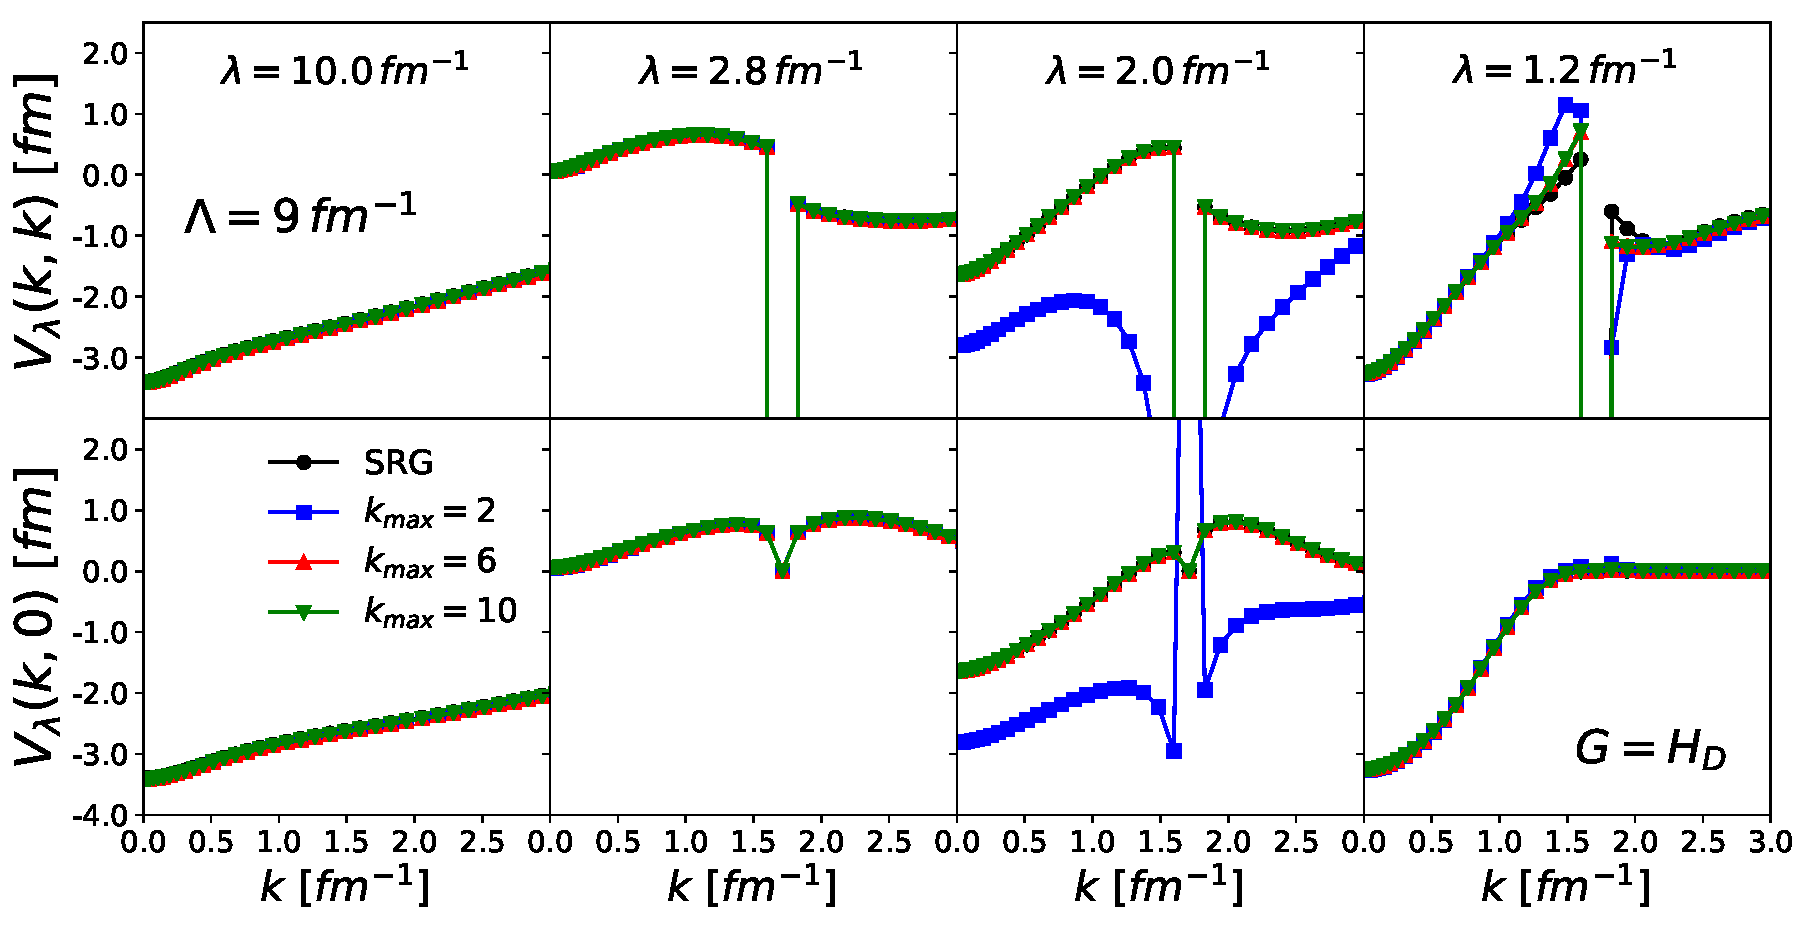
\includegraphics[clip,width=0.7\columnwidth]{Magnus/potential_diagonals_offdiags_kvnn901_Wegner}%
	\caption{Caption.}
	\label{fig:potential_slices_high_cutoffs_Wegner}
\end{figure}
%
\begin{figure}[H]
	\centering
	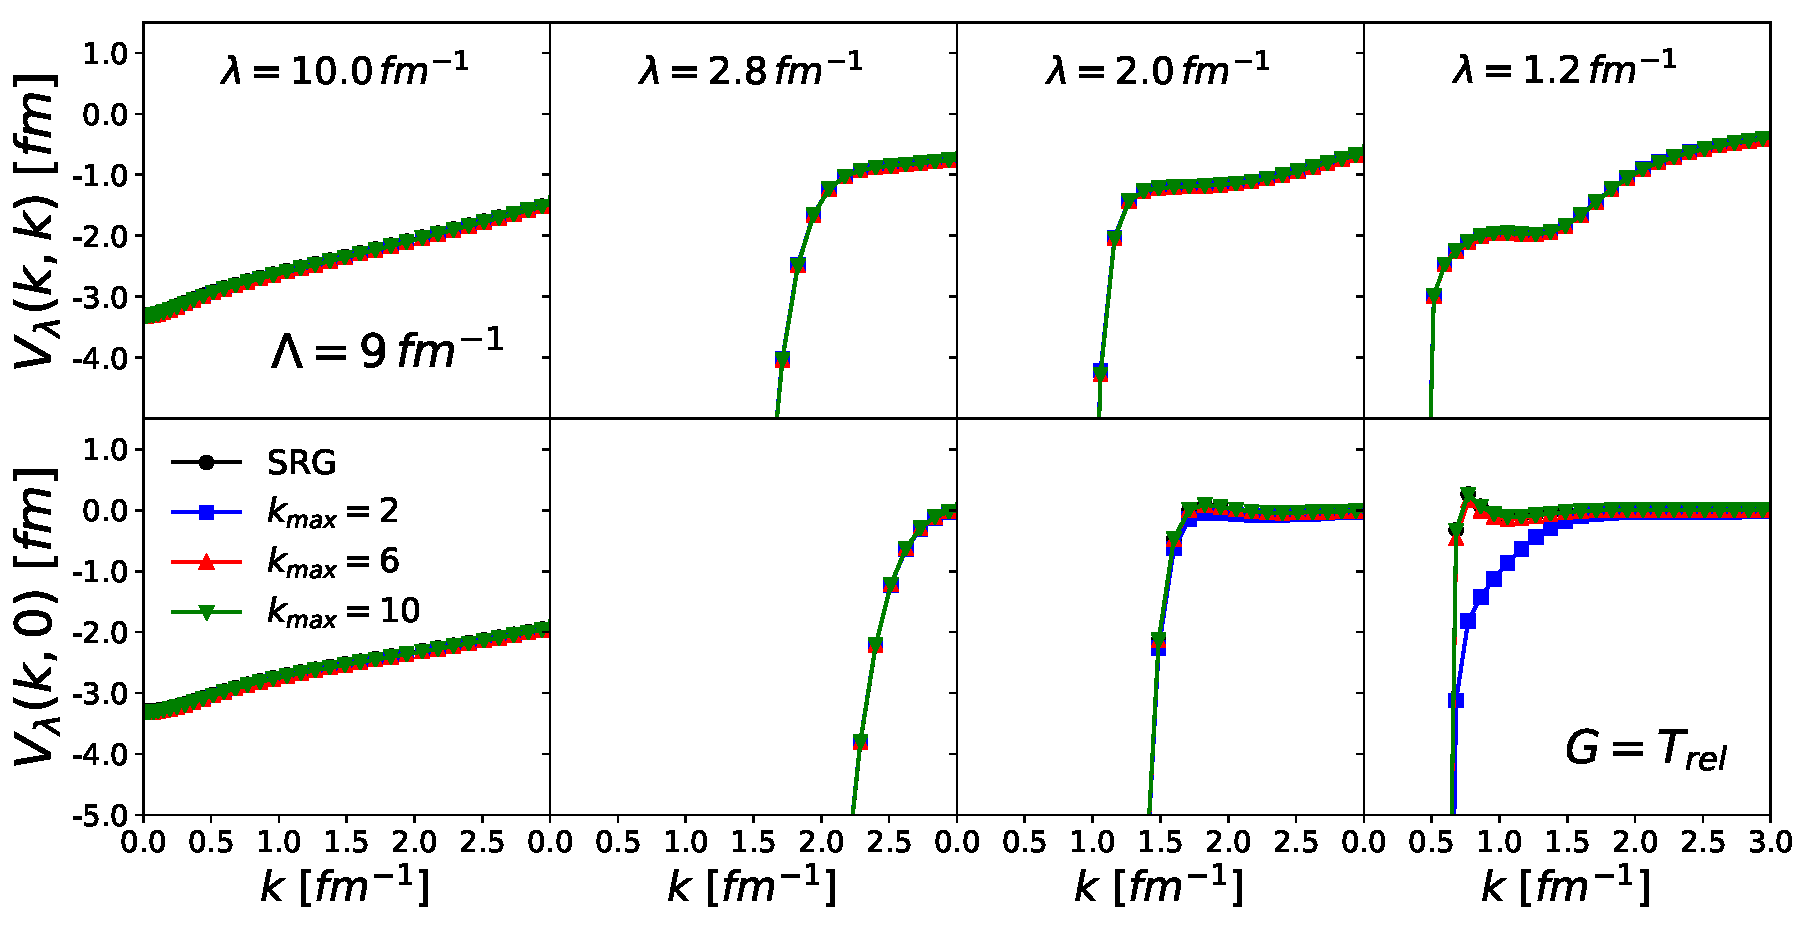
\includegraphics[clip,width=0.7\columnwidth]{Magnus/potential_diagonals_offdiags_kvnn901_T}%
	\caption{Caption.}
	\label{fig:potential_slices_high_cutoffs_T}
\end{figure}
%
%
\begin{table}
	\captionsetup{singlelinecheck=false,justification=raggedright}
	\caption{Relative error on the deuteron bound state energy and the root mean square of eigenvalues where $\tilde{\epsilon}$ denotes an eigenvalue of an SRG or Magnus-evolved Hamiltonian for $\Lambda=9 \, fm^{-1}$ and $\lambda=1.2 \, fm^{-1}$.}
	\label{tab:energies}
	\begin{ruledtabular}
		\begin{tabular}{{>{\centering\arraybackslash}m{1.5in}>{\centering\arraybackslash}m{1in}>{\centering\arraybackslash}m{1.5in}>{\centering\arraybackslash}m{2in}}}
      			$  $ & $G$ & $ |\frac{\epsilon_d-\tilde{\epsilon}_d}{\epsilon_d}| $ & $\sqrt{\frac{1}{N} \, \sum_{i}^{N} (\tilde{\epsilon}_i-\epsilon_i)^2}$   [MeV] \\
			\colrule
      			SRG & $ $ & $\num{1.165e-5}$ & $\num{3.016e-4}$ \\
      			Magnus, $k_{max}=2$ & $H_D$ & $\num{5.010e-10}$ & $\num{4.097e-9}$ \\
      			Magnus, $k_{max}=14$ & $ $ & $\num{1.206e-11}$ & $\num{3.950e-10}$ \\ \hline
      			SRG & $ $ & $\num{1.003e-4}$ & $\num{9.791e-5}$ \\
      			Magnus, $k_{max}=2$ & $T_{rel}$ & $\num{7.775e-8}$ & $\num{6.376e-8}$ \\
      			Magnus, $k_{max}=14$ & $ $ & $\num{7.607e-8}$ & $\num{6.359e-8}$ \\
		\end{tabular}
  	\end{ruledtabular}
\end{table}



%%%%%%%%%%%%%%%%%%%%%%%%%%%%%%%%%%%%%%%%%%%%%%%%%%%%%%%%%%%%%%%%%%%%%%%%%
\section{Evolution of other operators}
\label{sec:evolution_other_operators}


\noindent{%
-- SRG operator evolution for different potentials and generators.
}
\\
-- General questions to address: universality for operators, different generators.
\\
-- Give relevant equations. Unitary transformation equation.
\\
\textbf{Momentum projection operator}
\\
-- Relevant equations: just the momentum projection operator in momentum-space.
%
\begin{itemize}
	\item Contours and general behavior: SRG transformation shifts strength of operator to low-momentum.
	\item Deuteron momentum distributions. Why does this make sense with the transformed operators?
	\item Diagonals and far off-diagonals. Universality.
	\item Same questions but with figures of the integrand.
\end{itemize}
%
\begin{figure}[H]
	\centering
	\subfloat[]{%
	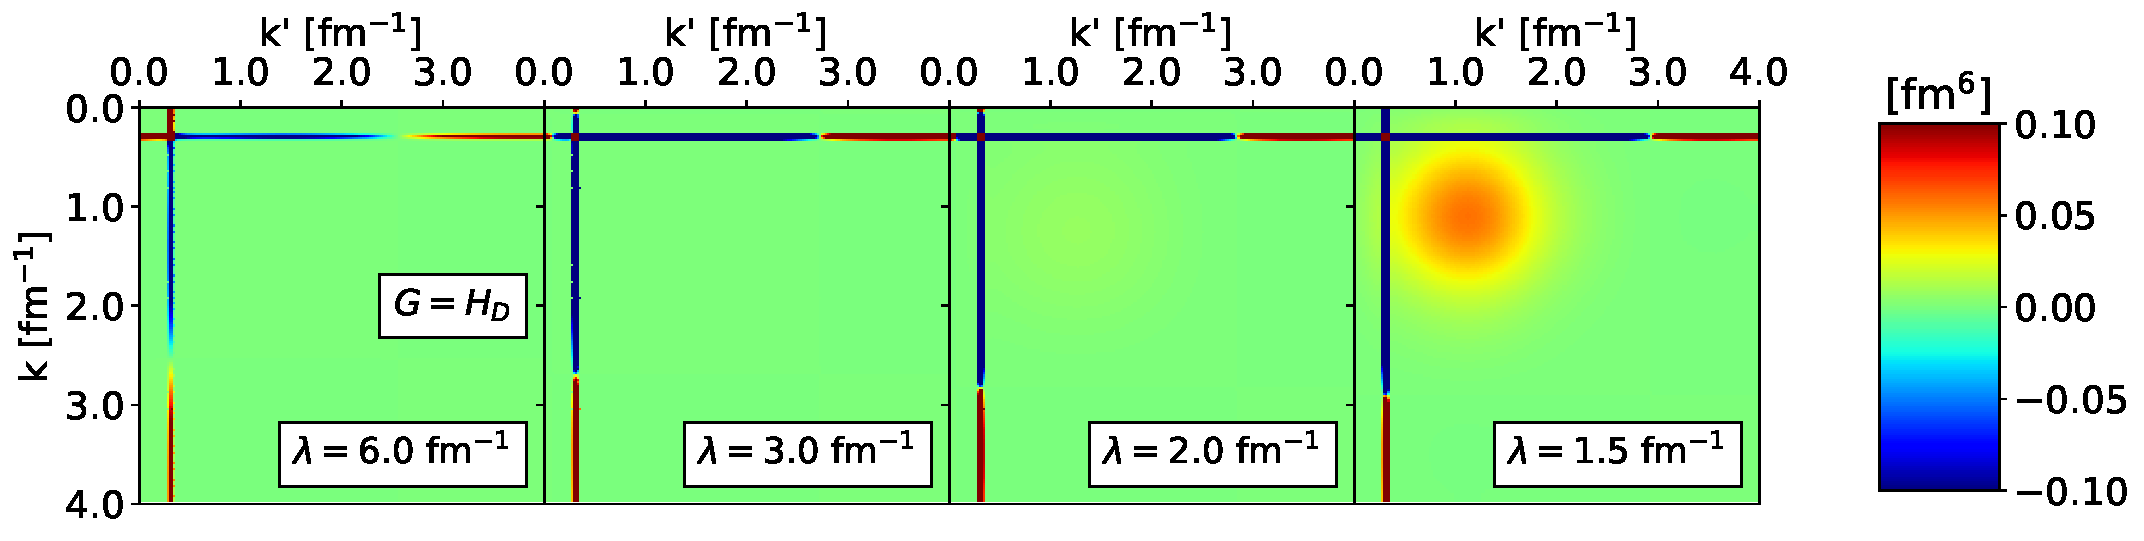
\includegraphics[clip,width=0.7\columnwidth]{SRG_operators/momentum_projection_contours_q0,30_kvnn111_3S1_Wegner}%
	}
	
	\subfloat[]{%
	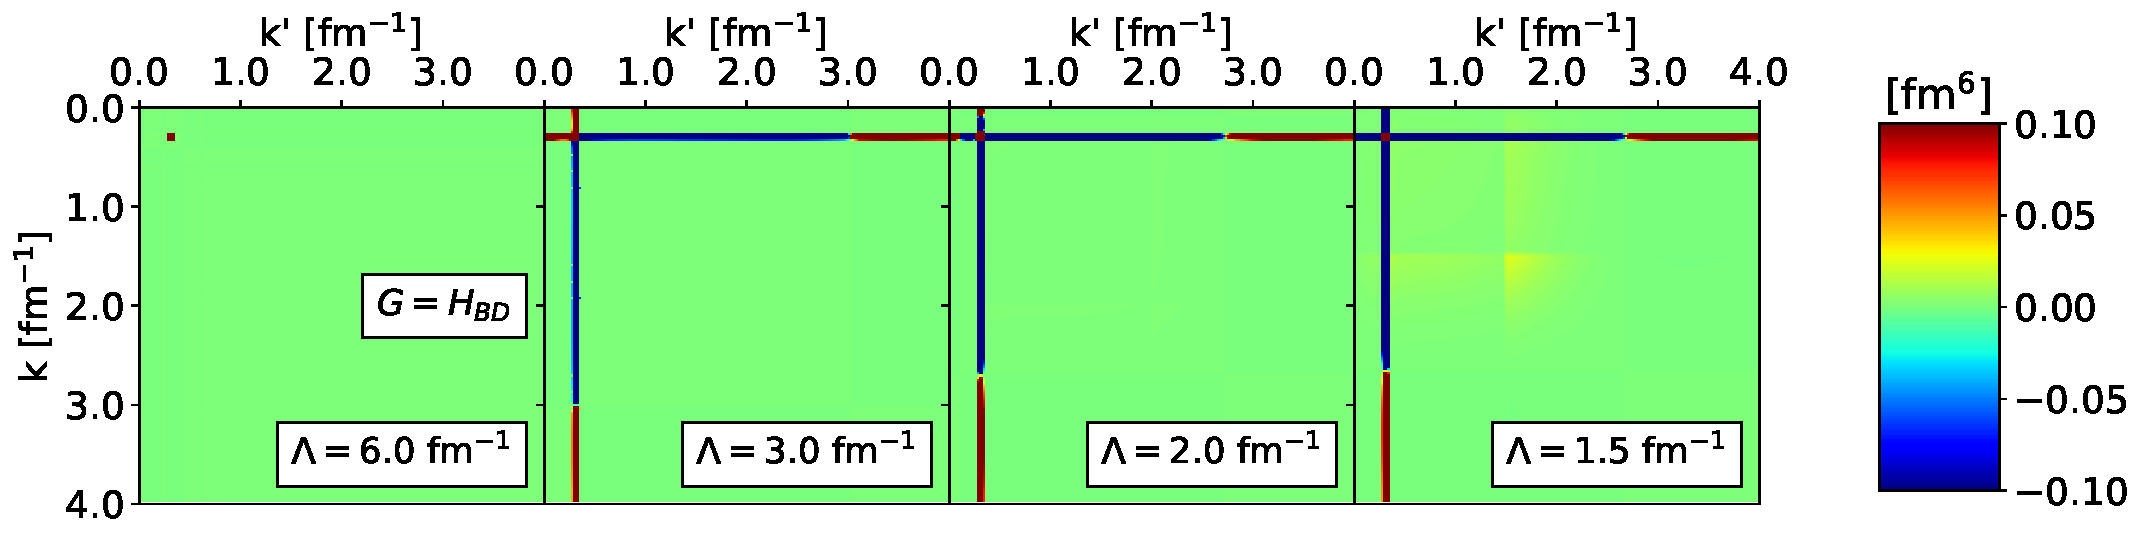
\includegraphics[clip,width=0.7\columnwidth]{SRG_operators/momentum_projection_contours_q0,30_kvnn111_3S1_Block-diag}%
	}
	\caption{Caption.}
	\label{fig:momentum_projection_contours_q0,30_3S1_RKE}
\end{figure}
%
\begin{figure}[H]
	\centering
	\subfloat[]{%
	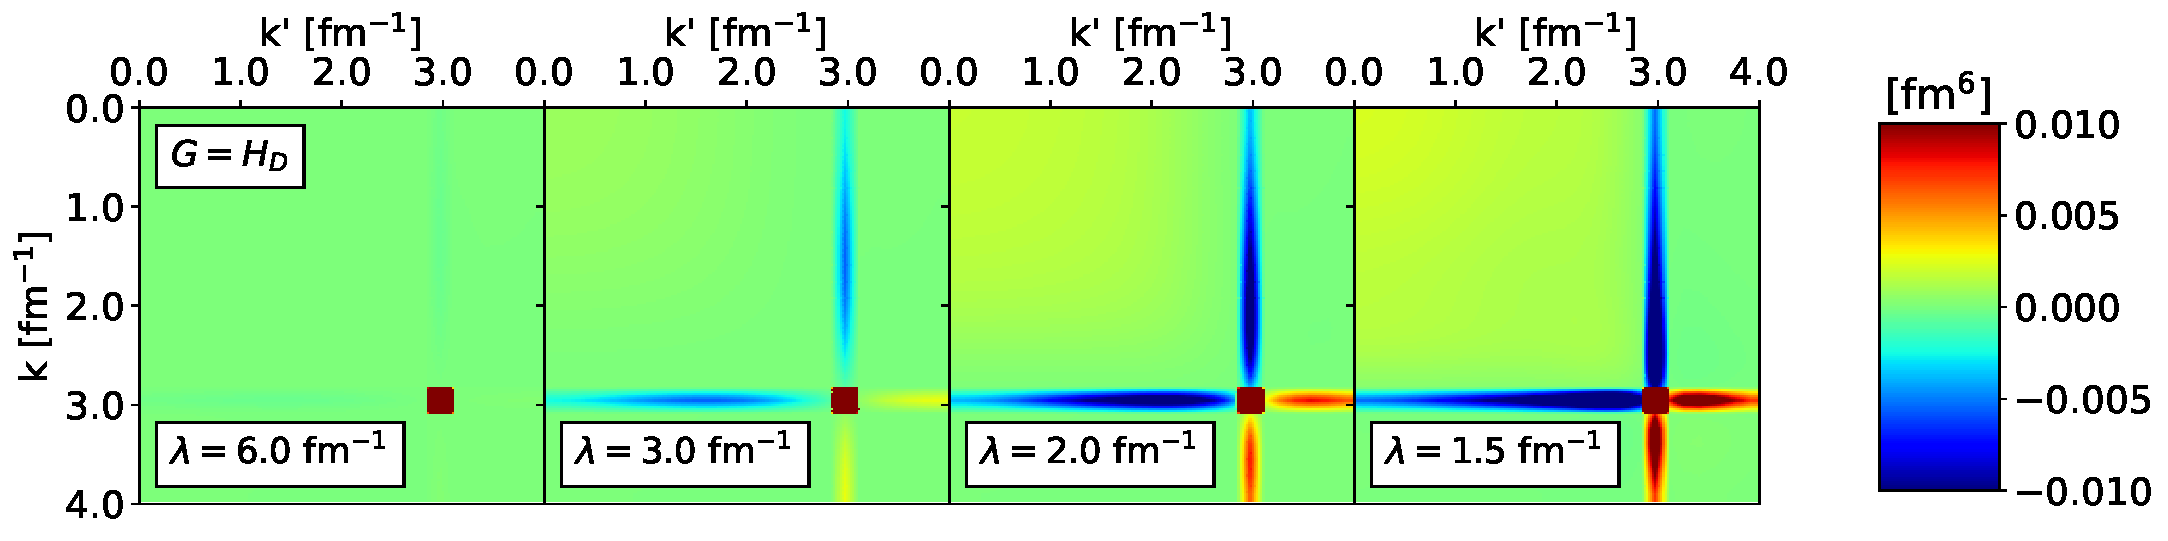
\includegraphics[clip,width=0.7\columnwidth]{SRG_operators/momentum_projection_contours_q3,00_kvnn111_3S1_Wegner}%
	}
	
	\subfloat[]{%
	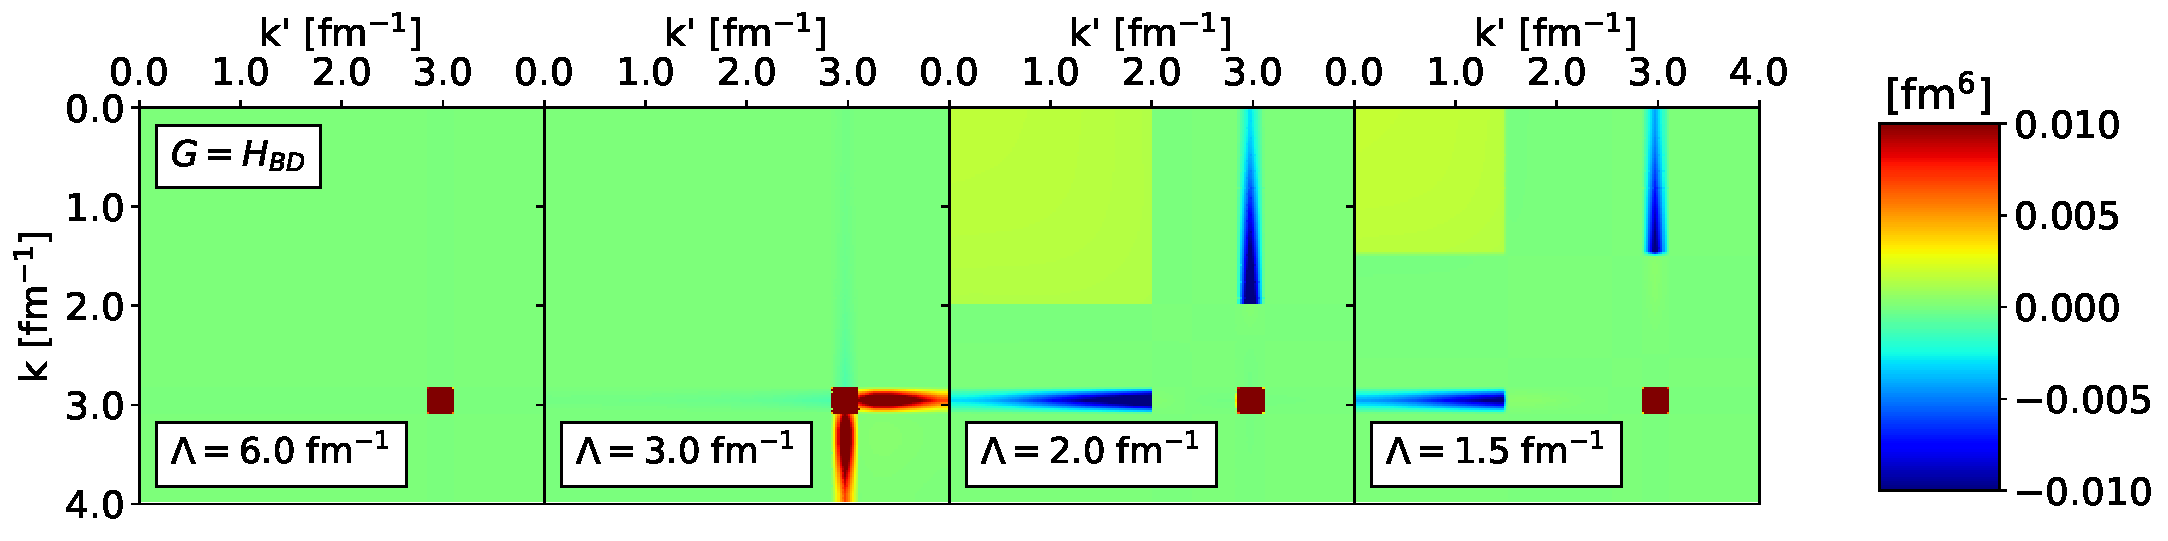
\includegraphics[clip,width=0.7\columnwidth]{SRG_operators/momentum_projection_contours_q3,00_kvnn111_3S1_Block-diag}%
	}
	\caption{Caption.}
	\label{fig:momentum_projection_contours_q3,00_3S1_RKE}
\end{figure}
%
\begin{figure}[H]
	\centering
	\subfloat[]{%
	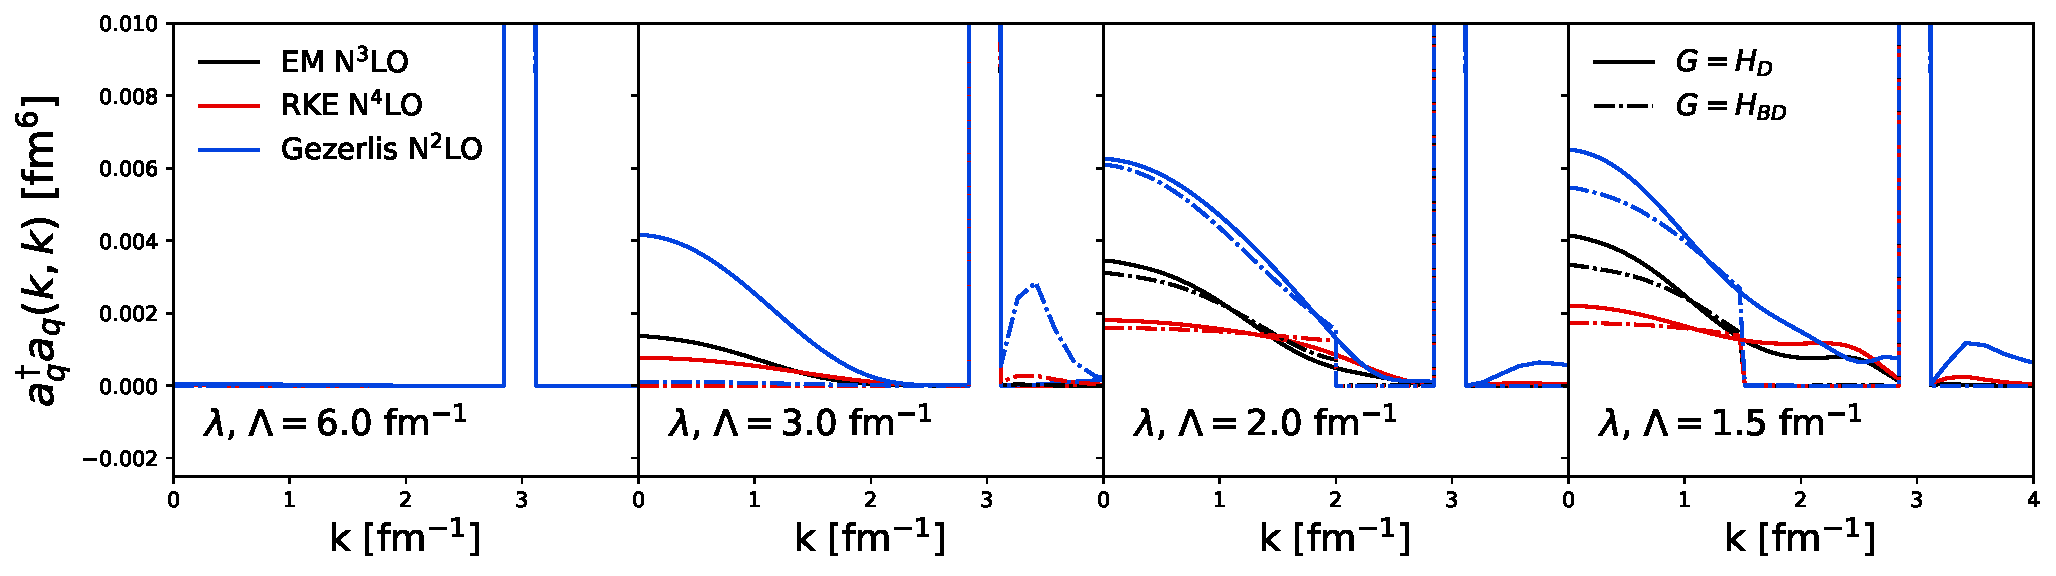
\includegraphics[clip,width=0.7\columnwidth]{SRG_operators/momentum_projection_diag_q3,00_3S1_kvnns_10_111_222_lamb1,5}%
	}
	
	\subfloat[]{%
	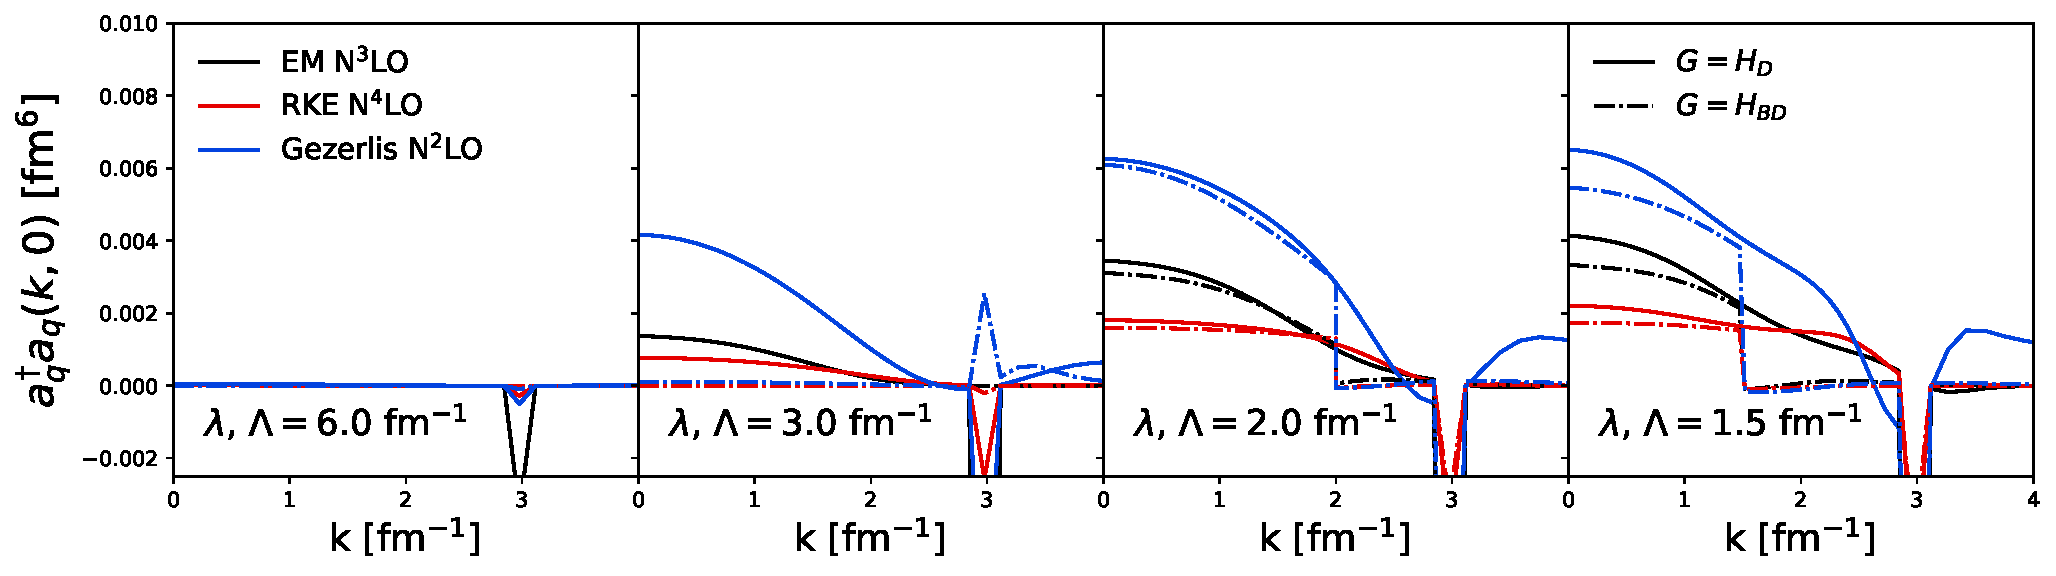
\includegraphics[clip,width=0.7\columnwidth]{SRG_operators/momentum_projection_off-diag_q3,00_3S1_kvnns_10_111_222_lamb1,5}%
	}
	\caption{Diagonal (a) and far off-diagonal (b) matrix elements of the momentum projection operator under SRG transformations with EM N$^3$LO (black), RKE N$^4$LO (red) and Gezerlis \textit{et al.}~N$^2$LO (blue) potentials evolving right to left with Wegner (solid) and block-diagonal (dashed) generators in the $^3$S$_1$ channel. Here, we use $\lambda$ for Wegner evolution and $\Lambda$ for block-diagonal evolution. For block-diagonal evolution, we fix $\lambda=1.5$ fm$^{-1}$.}
	\label{fig:momentum_proj_3S1}
\end{figure}
%
\begin{figure}[H]
	\centering
	\subfloat[]{%
	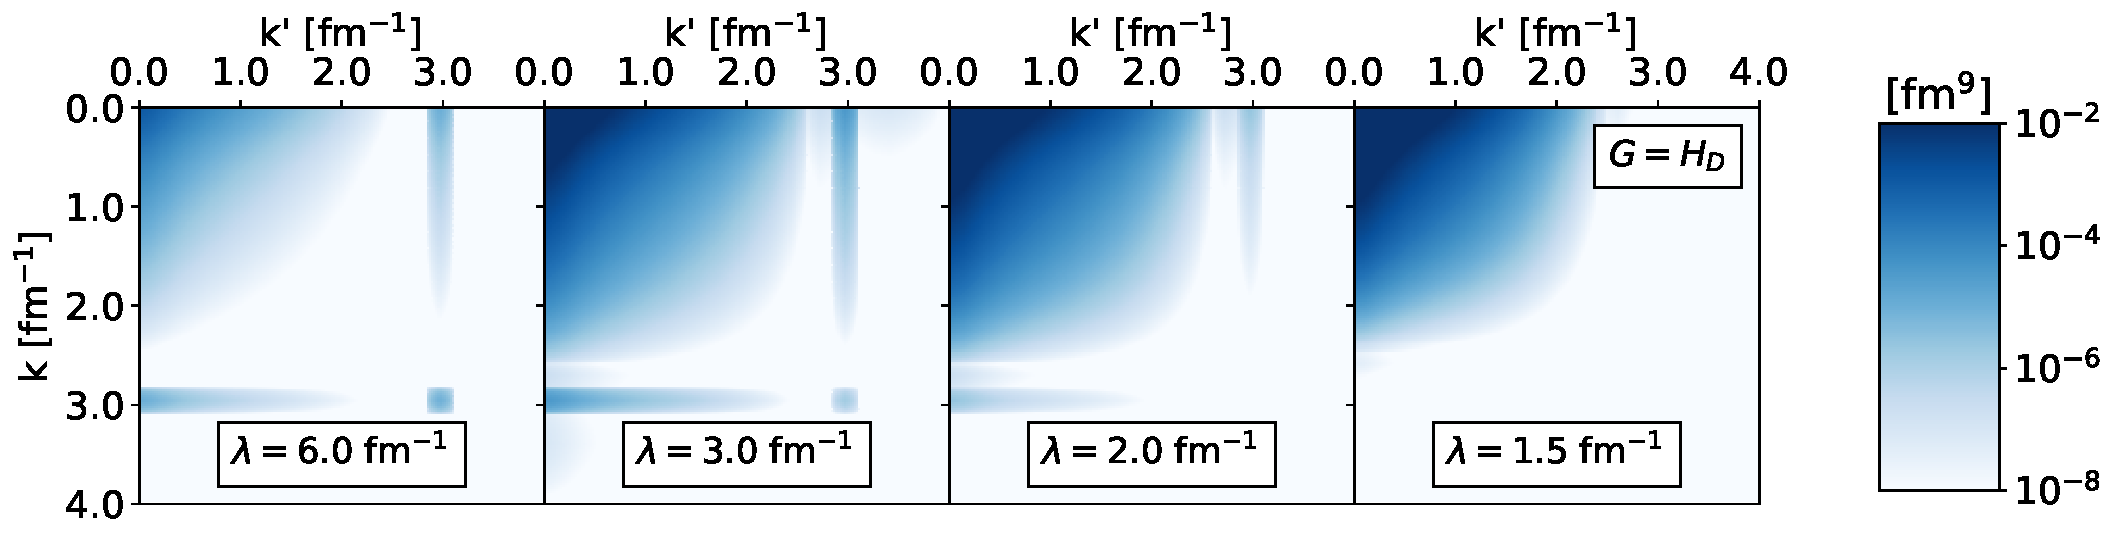
\includegraphics[clip,width=0.7\columnwidth]{SRG_operators/momentum_projection_integrand_contours_q3,00_kvnn111_Wegner}%
	}
	
	\subfloat[]{%
	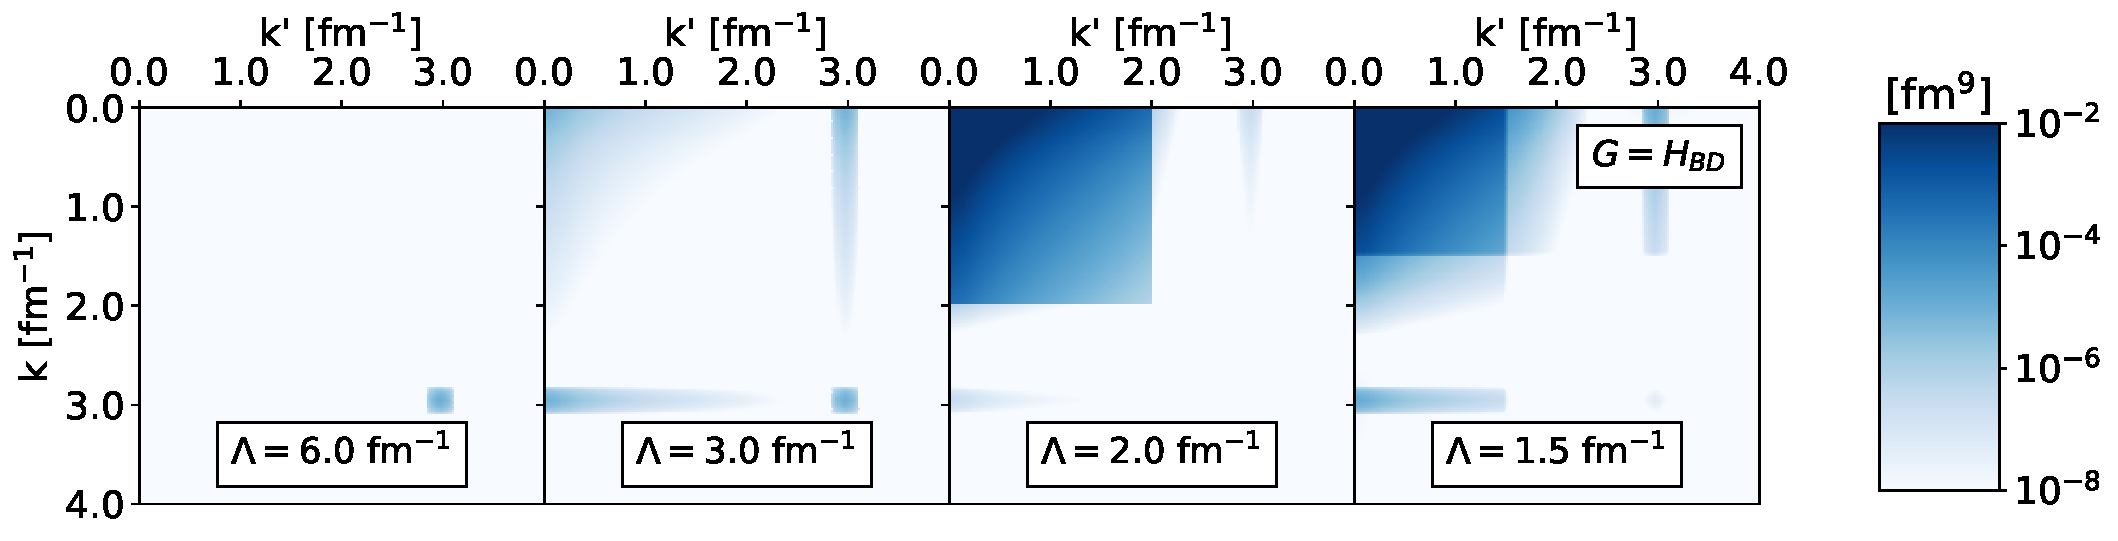
\includegraphics[clip,width=0.7\columnwidth]{SRG_operators/momentum_projection_integrand_contours_q3,00_kvnn111_Block-diag}%
	}
	\caption{Caption.}
	\label{fig:momentum_projection_integrand_contours_q3,00_RKE}
\end{figure}
%
\textbf{$\hat{r}^2$ operator}
\\
-- Relevant equations: operator in coordinate-space and Hankel transformation.
\\
-- Add continuum state momentum distributions and how to understand operator evolution.
%
\begin{figure}[H]
	\centering
	\subfloat[]{%
	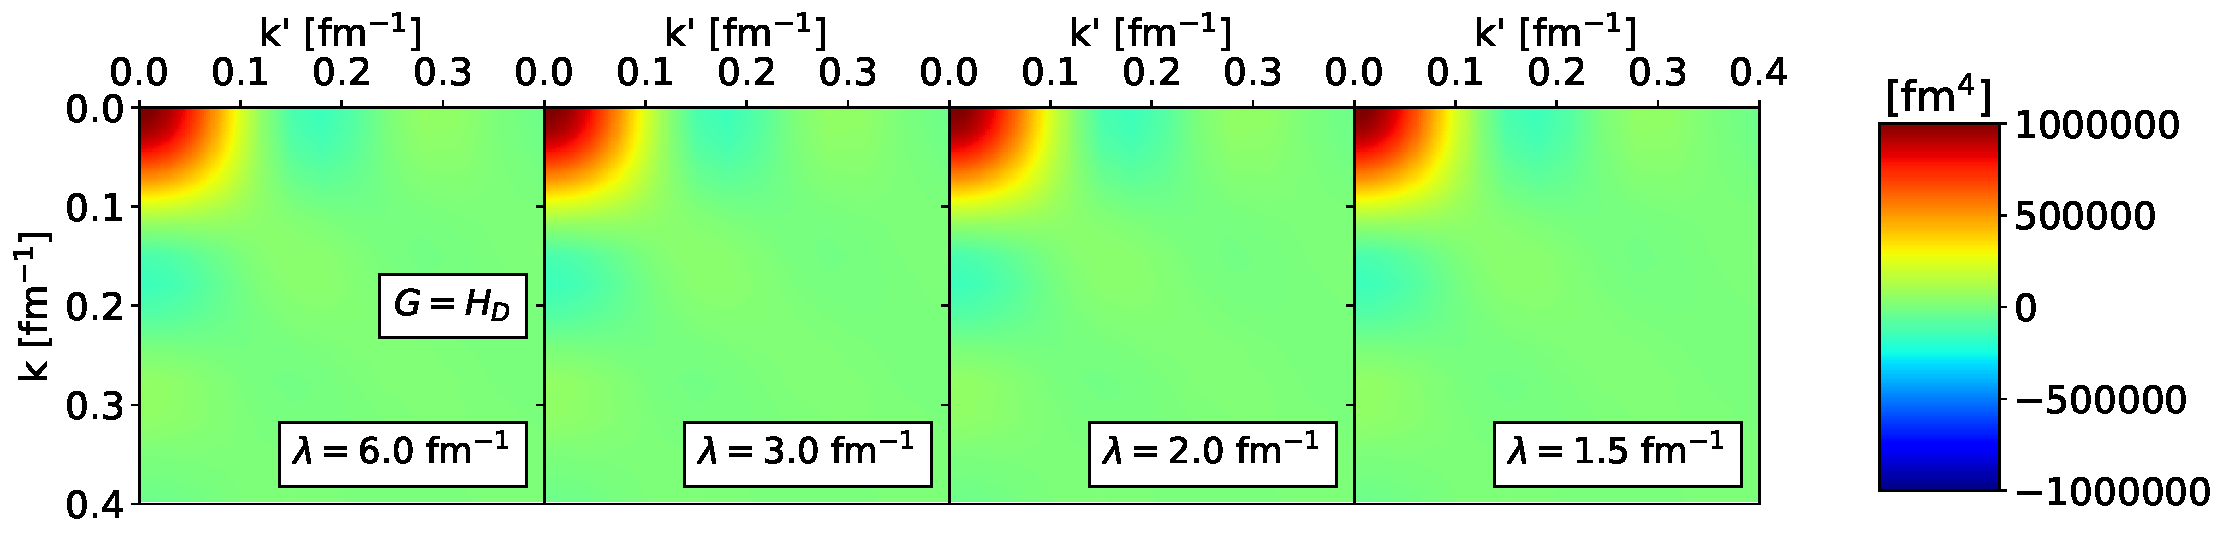
\includegraphics[clip,width=0.7\columnwidth]{SRG_operators/r2_contours_kvnn111_Wegner}%
	}
	
	\subfloat[]{%
	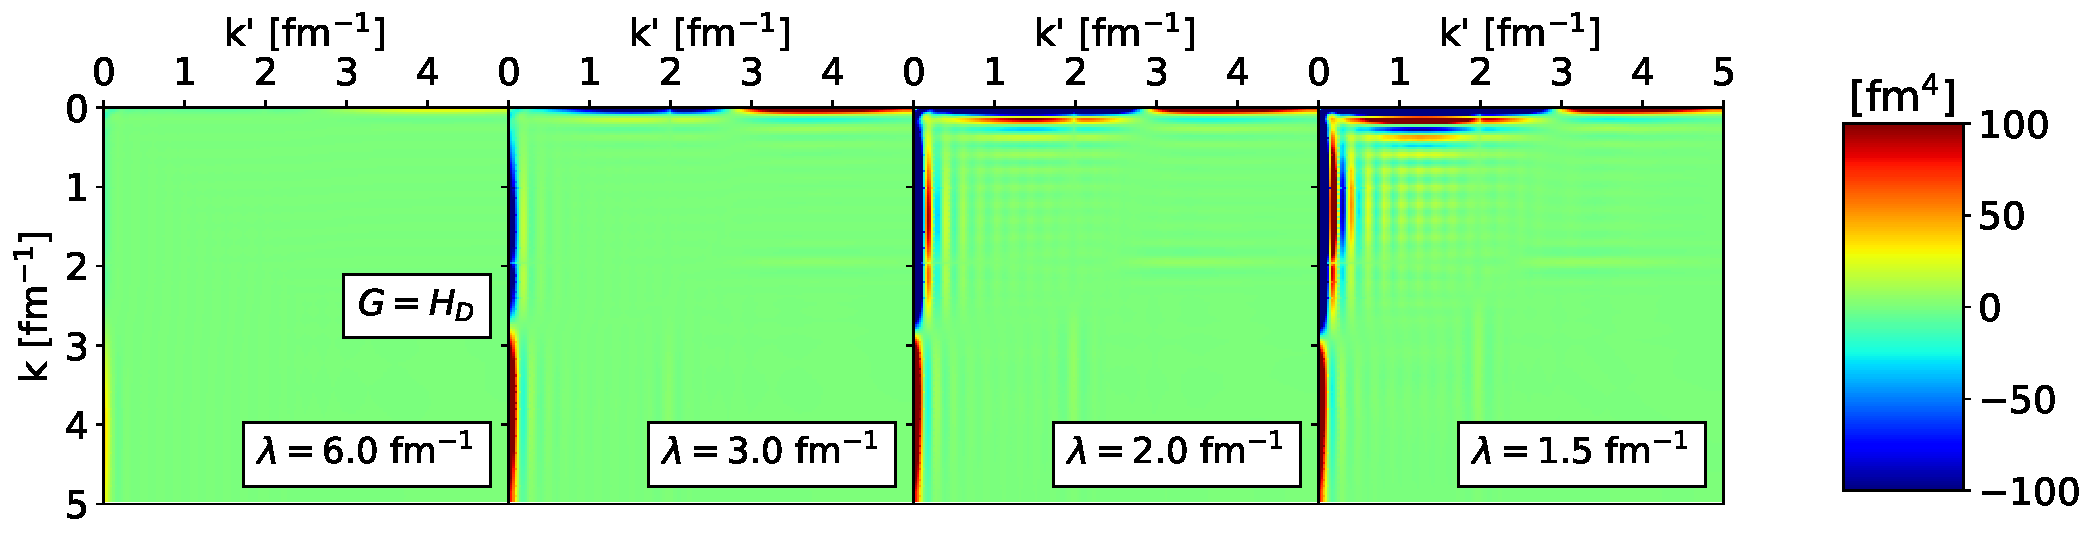
\includegraphics[clip,width=0.7\columnwidth]{SRG_operators/r2_diff_contours_kvnn111_Wegner}%
	}
	\caption{Caption.}
	\label{fig:r2_contours_RKE}
\end{figure}
%


%%%%%%%%%%%%%%%%%%%%%%%%%%%%%%%%%%%%%%%%%%%%%%%%%%%%%%%%%%%%%%%%%%%%%%%%%
\section{Conclusion}
\label{sec:conclusion}


\noindent{%
-- Summary.
}
\\
-- Outlook.


%%%%%%%%%%%%%%%%%%%%%%%%%%%%%%%%%%%%%%%%%%%%%%%%%%%%%%%%%%%%%%%%%%%%%%%%%


\bibliography{../tropiano_bib}

\end{document}